\documentclass{beamer}
% Language/Font package
\usepackage[utf8]{inputenc}
\usepackage[T1]{fontenc}

% Base package
\usepackage{graphicx}
\usepackage{color}
\usepackage{listings}
\usepackage{hyperref}
\usepackage{todonotes}

\usepackage{comment}

\usetheme[progressbar=frametitle]{metropolis}

\definecolor{links}{HTML}{2A1B81}
\hypersetup{colorlinks,linkcolor=,urlcolor=links}

\usepackage[french]{babel}

% Title
\title{Présentation Git}
\subtitle{Un outil de collaboration puissant}
\date{1\ier Mars 2018}
\author{Gaëtan Cassiers \and Alexandre Fiset \and Pierre Ortegat}
\institute{KAP Louvain-li-Nux}
\titlegraphic{\hfill\includegraphics[height=2cm]{img/logo.png}}

\begin{document}

% slides pré-atelier pour les personnes en avance
\begin{frame}
\begin{center}
  Suivez cette présentation sur votre ordinateur :

  \fbox{\Large\url{https://louvainlinux.org/atelier-git}}
\end{center}

Préparez-vous à utiliser \texttt{git} :
vous utiliserez le logiciel GitHub Desktop durant cette présentation.

Prenez un peu d'avance, installez-le:
\begin{itemize}
    \item Sur les ordinateur Windows UCL: installez
            \url{https://desktop.github.com}
    \item Ou installez GitHub Desktop sur votre ordinateur :
    \begin{itemize}
        \item \textbf{Ubuntu} : {\footnotesize{\url{https://github.com/shiftkey/desktop/releases}}}
        \item \textbf{Windows ou OS X} : \url{https://desktop.github.com}
    \end{itemize}
\end{itemize}
\end{frame}


\maketitle

\begin{frame}{Cette présentation}
    \begin{itemize}
        \item Cette présentation est sous license libre CC-BY 4.0.
        \item En ligne (slides en pdf et sources \LaTeX, exercices\ldots):
            \url{https://github.com/louvainlinux/atelier-git}
    \end{itemize}
\end{frame}

\begin{frame}{Table des matières}

\setbeamertemplate{section in toc}[sections numbered]
\tableofcontents[hideallsubsections]

\end{frame}

\section{Introduction}

\begin{frame}{Gérer un projet}
Comment gérez-vous actuellement un projet ?

\begin{itemize}
    \item L'envoyer à travers un message sur Facebook, ... (\textbf{Très mauvaise idée})
    \item L'envoyer par mail (\textbf{Un peu moins})
    \item Utiliser une Dropbox, Google Drive, ... (\textbf{Déjà mieux mais toujours risqué ou manque de fonctionnalités})
\end{itemize}

Solution : Utiliser un \textbf{système de gestion de version décentralisé}
(Distributed Version Control System (DVCS) pour les anglophiles).
\end{frame}

\begin{frame}{Un DVCS ?}
    \begin{itemize}
        \item \textbf{Version} Enregistre des \og{}instantanés\fg{} du projet.
        \item \textbf{Gestion} Revenir en arrière, voir des différences,
            fusionner des modifications.
        \item \textbf{Décentralisé} Chacun
            \begin{itemize}
                \item a sa copie (avec son historique) sur son PC,
                \item peut mettre sa copie (et son historique) en ligne,
                \item peut récupérer sur son PC les copies et historiques disponibles en ligne,
                \item peut fusionner différentes copies (semi-)automatiquement.
            \end{itemize}
        \item \textbf{Projet} n'importe quel répertoire (\og dossier\fg) sur votre ordinateur. Donc
            n'importe quoi : Bureautique, \LaTeX, code, images, musique\dots
    \end{itemize}
\end{frame}

\begin{frame}{Et Git dans tout ça ?}
\texttt{Git} a été créé en 2005 par Linus Torvalds (auteur de
\texttt{Linux}); le plus connu et utilisé.

À l'origine, interface en ligne de commande.

Aujourd'hui: aussi des interfaces graphiques, dont GitHub Desktop.
\end{frame}

\begin{frame}{Mais on m'avait parlé de GitHub !}
    Souvenez-vous...
    \begin{itemize}
        \item \textbf{Décentralisé} Chacun
            \begin{itemize}
                \item peut mettre sa copie (et son historique) en ligne,
                \item \dots
            \end{itemize}
    \end{itemize}

    Il y a plein d'"endroits" en ligne o\`u on peut envoyer son travail, GitHub
    est le plus connu.

    En plus de ça, GitHub a des fonctionnalités pour interagir avec des collaborateurs.
\end{frame}

\section{Principes de Git}

\begin{frame}{Concepts}
    \begin{itemize}
        \item \textbf{Espace de travail:}
            les fichiers, répertoires... dans lesquels on
            travaille. Ils n'ont rien de spécial par rapport à d'autres dossiers
            sur l'ordinateur.
        \item \textbf{Dépôt:} espace de travail + historique, sur un ordinateur.
        \item \textbf{Commit:} "version", est le successeur d'une autre commit.
        \item \textbf{Historique:} la "chaîne" de tous les commits, du plus ancien au plus récent.
        \item \textbf{Dépôt distant:} un dépot qui se trouve chez GitHub.
    \end{itemize}
\end{frame}

\begin{frame}
\frametitle{Concept: le \textbf{commit}}

\begin{center}
    \includegraphics[width=0.9\textwidth]{img/commits.png}
\end{center}
\footnotesize{Les illustrations non-sourcées viennent de \url{https://git-scm.com/book}.}
\end{frame}

\begin{frame}{Actions}
    \begin{itemize}
        \item \textbf{Créer} un dépot sur GitHub.
        \item \textbf{Cloner} (faire une copie d') un dépot de GitHub sur son PC.
        \item \textbf{Modifier/créer} des fichiers (pas avec Git !).
        \item \textbf{Ajouter} un fichier modifié: il sera pris en compte dans le
            prochain commit.
        \item \textbf{Faire un commit}: créer une nouvelle version, qui contient tous
            les fichiers ajoutés. On y ajoute un commentaire (qui décrit les
            changements).
        \item \textbf{Consulter} un historique.
        \item \textbf{Push}: envoyer ses nouveaux commits sur GitHub.
        \item \textbf{Pull}: récupérer des changements (qui ont été envoyés
            par quelqu'un d'autre) depuis GitHub.
        \item \textbf{Merge}: quand on Pull et qu'on a aussi des nouveaux commits sur
            son PC. Git essaye de fusionner automatiquement; s'il ne sait pas
            le faire, il demande à l'utilisateur.
    \end{itemize}
\end{frame}

\begin{frame}[standout]
    Questions ?
\end{frame}


\section{Utilisation: en pratique}

\begin{frame}{Créer un dépot sur GitHub}
    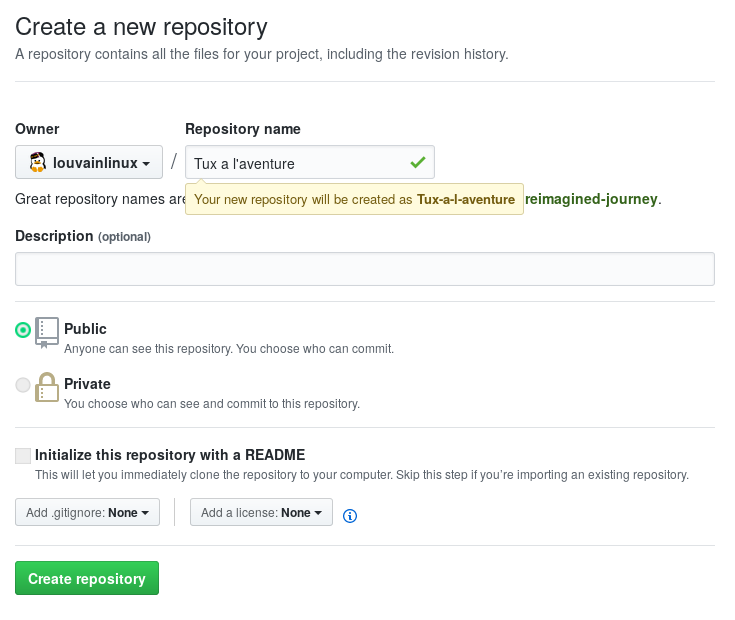
\includegraphics[width=.9\textwidth]{img/github_desktop/new_repo.png}
\end{frame}

\begin{frame}{Ajouter un collaborateur sur GitHub}
    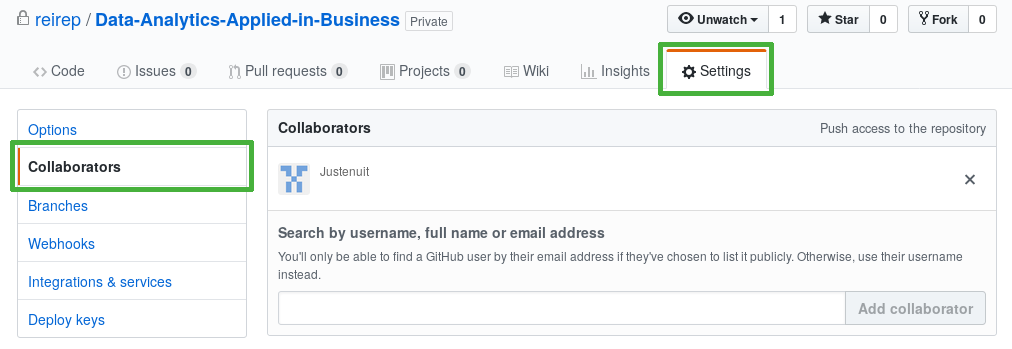
\includegraphics[width=\textwidth]{img/github_desktop/colaborator.png}
\end{frame}

\begin{frame}{Cloner un dépot sur son PC}
    Deux étapes:
    \begin{enumerate}
        \item Prendre l'url du dépôt sur Github
        \item Donner l'url à Github desktop
    \end{enumerate}
    \begin{columns}    
        \begin{column}{0.5\textwidth}
            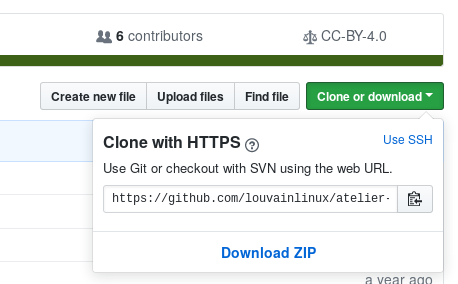
\includegraphics[width=.9\textwidth]{img/github_desktop/clone_repo.png}\\ $ $\\
        \end{column}
        \begin{column}{0.5\textwidth}
            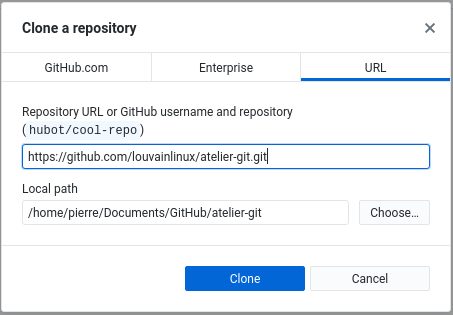
\includegraphics[width=.9\textwidth]{img/github_desktop/clone_repo_desktop_2.png}\\
            {\small Pour ouvrir cette fenêtre : \\File $\rightarrow$ Clone repository}
        \end{column}
    \end{columns}
    \begin{center}
        Ne pas effacer le \emph{".git"} !
    \end{center}
\end{frame}

\begin{frame}{Ajouter des fichiers}
    \begin{center}
        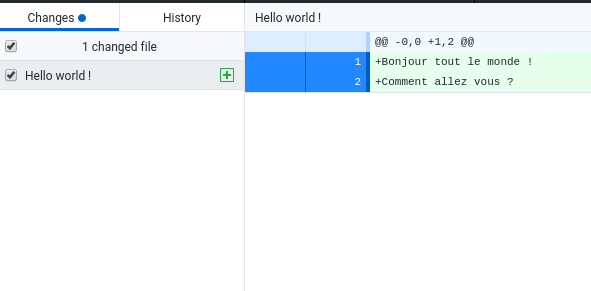
\includegraphics[width=\textwidth]{img/github_desktop/see_added.png}
    \end{center}
\end{frame}

\begin{frame}{Remarque: fichier texte vs binaire}
    \begin{itemize}
        \item Fichiers texte: programme, \LaTeX\dots\\
            \begin{center}
                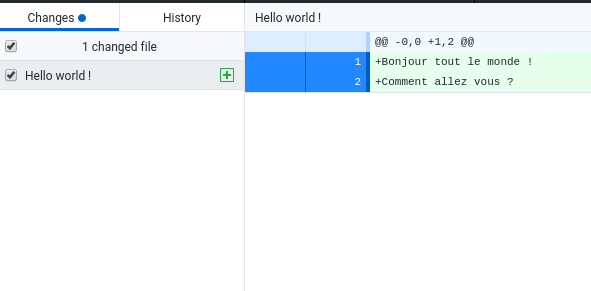
\includegraphics[width=.75\textwidth]{img/github_desktop/see_added.png}\\
            \end{center}
        \item Fichiers binaires: le reste: Word, Writer, images, sons, PDF\dots\\
            \begin{center}
                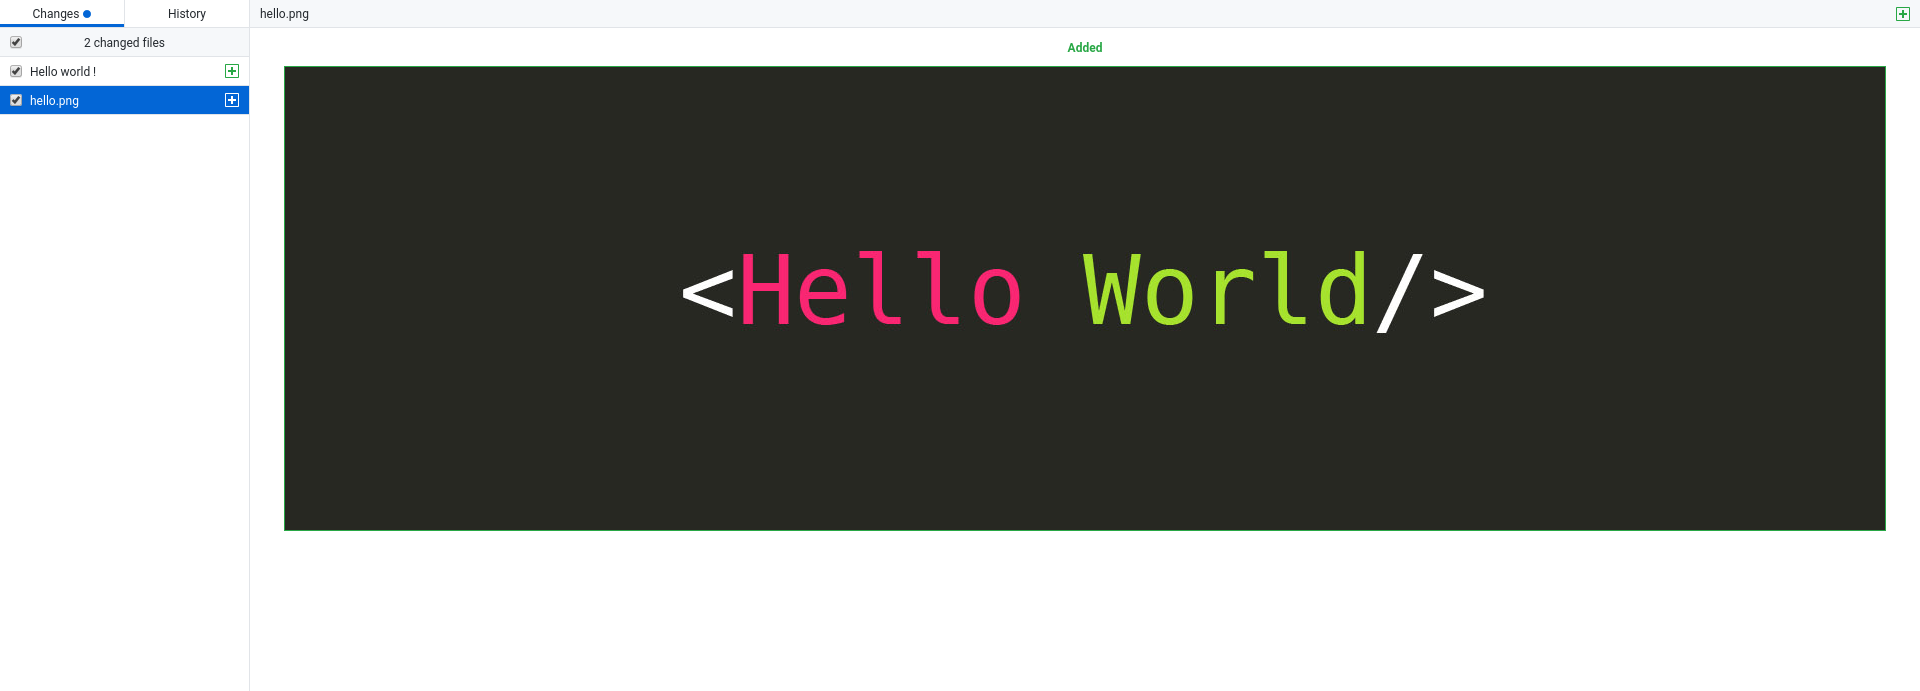
\includegraphics[width=.75\textwidth]{img/github_desktop/binary_file.png}
            \end{center}
    \end{itemize}
\end{frame}

\begin{frame}{Créer un dépôt local}
    \begin{center}
        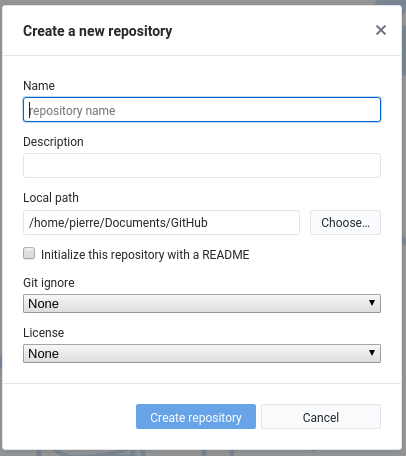
\includegraphics[scale=0.45]{img/new_repo.png}
    \end{center}
\end{frame}

\begin{frame}{Créer un commit}
\begin{itemize}
    \item Créer un \texttt{commit} sur base des fichiers ajoutés.
    \item Message de \texttt{commit}: décrit les changements effectués.
\end{itemize}
\begin{center}
    
\includegraphics[width=.5\textwidth]{img/github_desktop/commit.png}
\end{center}
\end{frame}

\begin{frame}{Visualiser l'historique}
    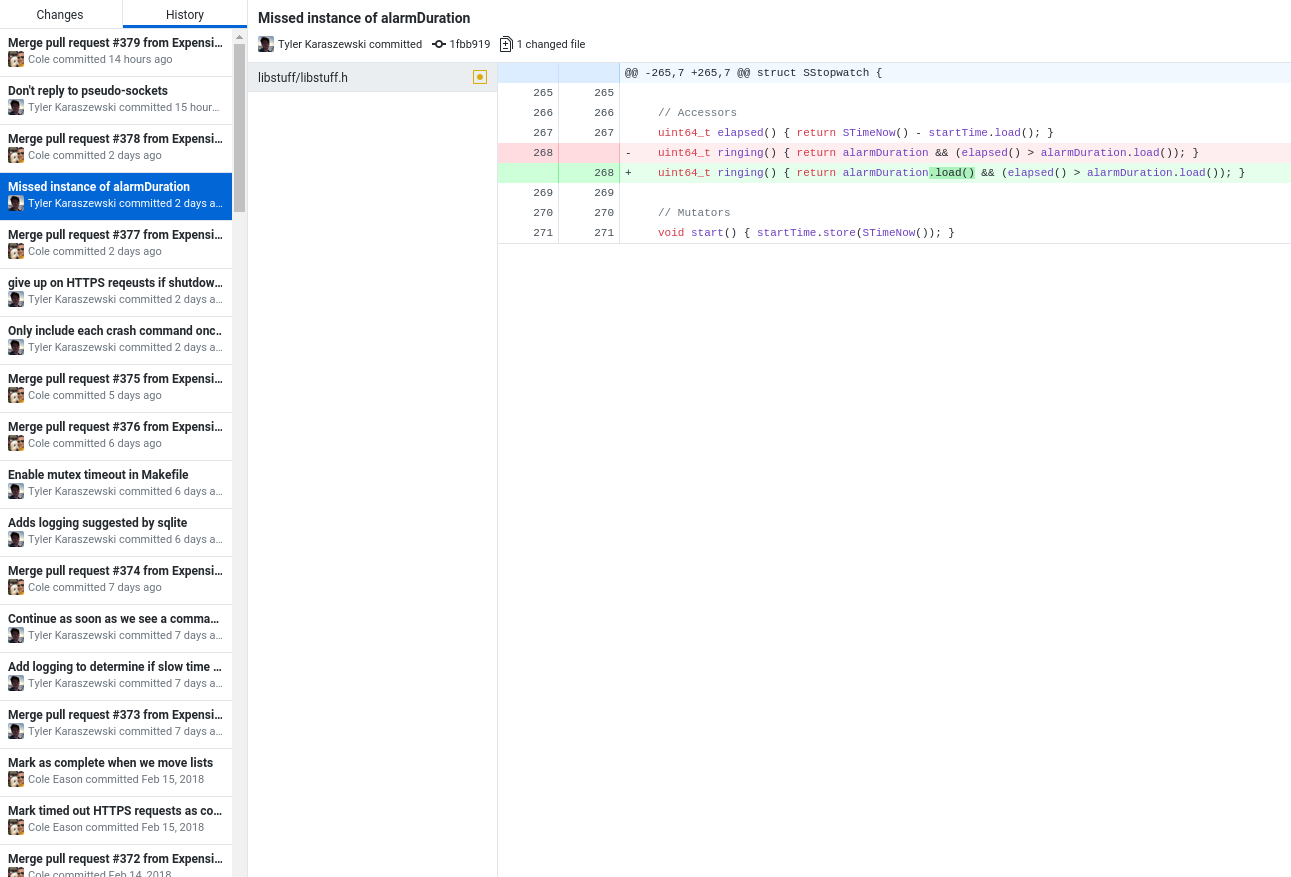
\includegraphics[width=.9\textwidth]{img/github_desktop/historique.png}
\end{frame}

\begin{frame}{Astuce: ignorer des fichiers}
    Des fichiers que vous ne voulez jamais dans Git (résultats de compilation,
    fichiers temporaires\dots) ? Cachez-les !

    NB: Cela crée un fichier \texttt{.gitignore}: celui-là, on le versionne.
    \begin{center}
        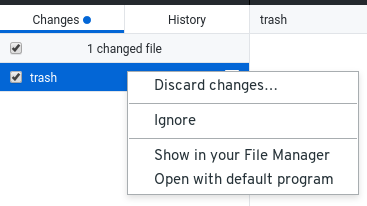
\includegraphics[width=.5\textwidth]{img/github_desktop/ignore.png}
    \end{center}
\end{frame}

\begin{frame}{Push: envoyer des commits sur GitHub}
    \begin{center}
        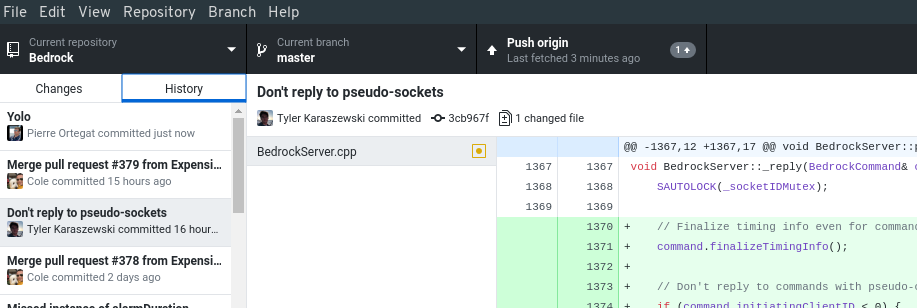
\includegraphics[width=\textwidth]{img/github_desktop/push_2.png}
    \end{center}
\end{frame}

\begin{frame}{Pull: récupérer des commits qui sont sur GitHub}
    \begin{center}
        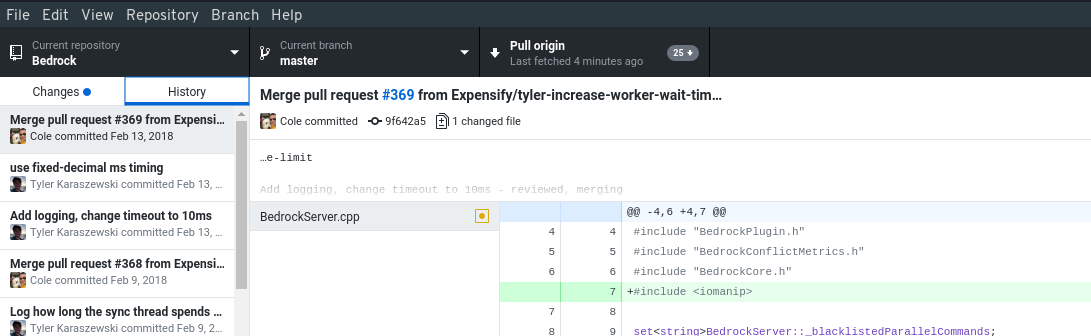
\includegraphics[width=\textwidth]{img/github_desktop/pull_2.png}
    \end{center}
\end{frame}

\begin{frame}{Merge non-automatique: quand il y a des conflits}
    Message d'erreur:
    \begin{center}
        
\includegraphics[width=.9\textwidth]{img/github_desktop/conflit_1.png}
    \end{center}
\end{frame}

\begin{frame}{Merge non-automatique: quand il y a des conflits}
    Trouver le(s) fichier(s) en conflit:
    \begin{center}
        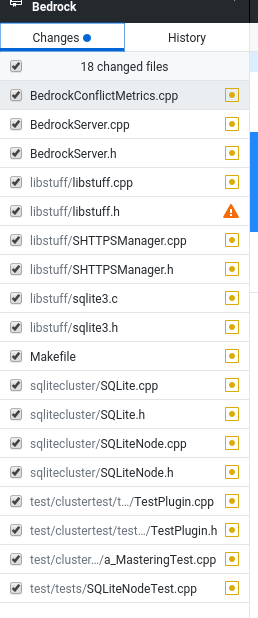
\includegraphics[width=.27\textwidth]{img/github_desktop/conflit_2.png}
    \end{center}
\end{frame}

\begin{frame}{Merge non-automatique: quand il y a des conflits}
    Trouver le(s) endroit(s) en conflit dans le fichier (reconnaissables par des balises) :

    Avant: 
    \begin{center}
        
\includegraphics[width=\textwidth]{img/github_desktop/merge_before.png}
    \end{center}

    Après:
    \begin{center}
        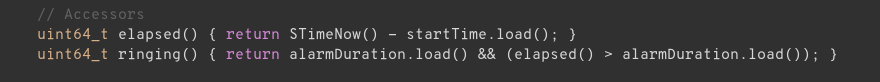
\includegraphics[width=\textwidth]{img/github_desktop/merge_after.png}
    \end{center}
\end{frame}

\begin{frame}{Merge non-automatique: quand il y a des conflits}
    Choisir la version que l'on veut garder et commit:\\
    \begin{center}
        
\includegraphics[width=.3\textwidth]{img/github_desktop/conflit_4.png}\\
        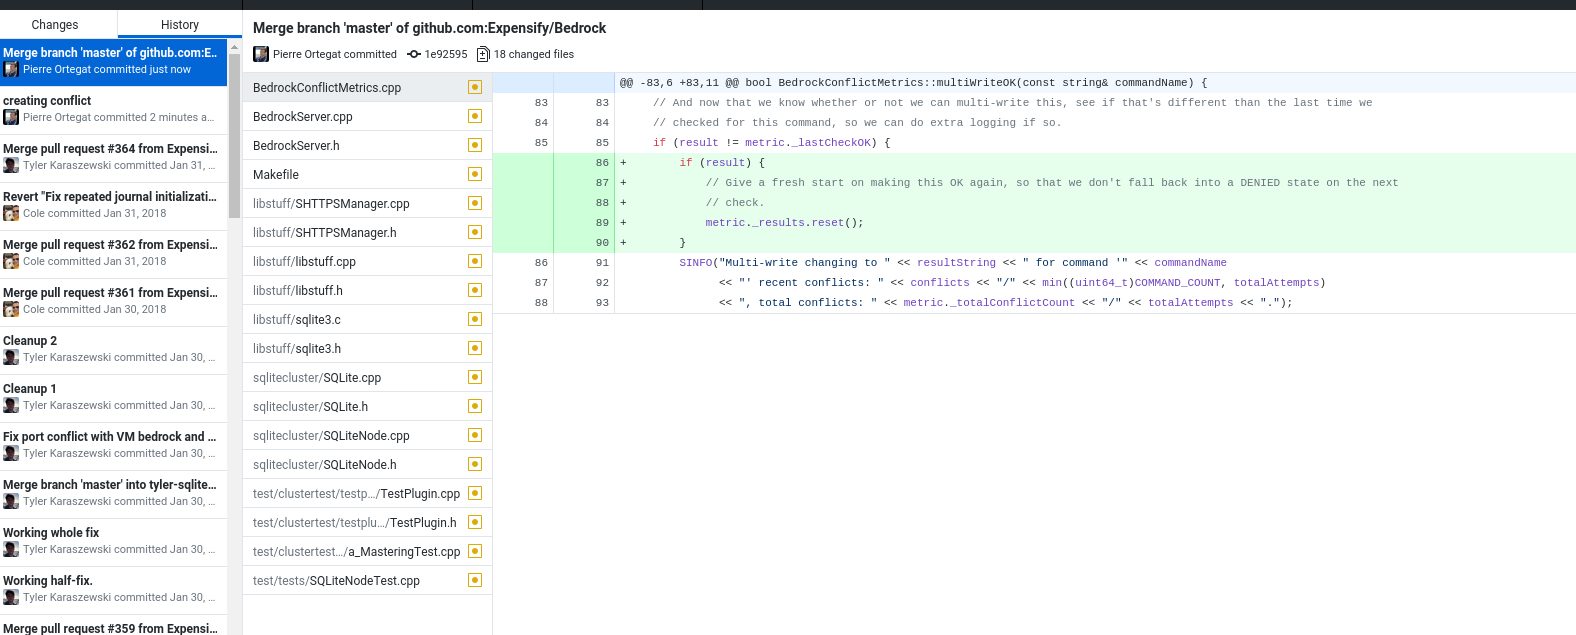
\includegraphics[width=.95\textwidth]{img/github_desktop/conflit_5.png}
    \end{center}
\end{frame}

\begin{frame}{Astuce: de l'aide !}
    On peut trouver de l'aide:
    
    \begin{center}
    	Github help:\\ \url{https://help.github.com/}
    \end{center}
    \begin{center}
        Github desktop help:\\ \url{https://help.github.com/desktop/}
    \end{center}
\end{frame}


\section{Installation et configuration}

\begin{frame}[label = {instal}]{Installer GitHub desktop}
\begin{itemize}
    \item Sur les ordinateur Windows UCL: installez
            \url{https://desktop.github.com}
    \item Ou installez GitHub Desktop sur votre ordinateur :
    \begin{itemize}
        \item \textbf{Ubuntu} : {\footnotesize{\url{https://github.com/shiftkey/desktop/releases}}}
        \item \textbf{Windows ou OS X} :
            \url{https://desktop.github.com}
    \end{itemize}
\end{itemize}
\end{frame}

\begin{frame}{Configuration de base}

Git a besoin de deux informations de base sur vous pour pouvoir travailler
efficacement :

\begin{itemize}
\item \textbf{Nom et Prénom}
\item \textbf{Email}
\end{itemize}

%L'option \lstinline{--global} permet de configurer \texttt{git} pour tous vos autres projets sur votre PC.
\end{frame}

%\begin{frame}{Configuration de base -- Éditeur de textes}
%    \textbf{Linux}
%    \textbf{Windows}
%    \textbf{Mac}
%    TODO: screenshots
%    
%    Pas besoin avec git desktop
%\end{frame}


\section{Exercices}
\subsection{Exercice 1}
\begin{frame}{Exercice 1 : partie 1}
Exercice à faire par \textbf{groupe de 2 ou 3}:

Pour tout le monde:
\begin{itemize}
    \item Créez un compte sur \href{https://github.com}{GitHub}.
\end{itemize}
Une personne du groupe:
\begin{itemize}
    \item Créez un dépôt nommé \textit{blagues} sur votre compte GitHub. Cocher la case "Initialize this repository...".
    \item Ajoutez les autres en collaborateurs sur le dépôt. Ils reçoivent
        une invitation par mail, ils doivent l'accepter.\footnote{Si vous arrivez sur une page 404, connectez-vous à github et ré-essayez.}
\end{itemize}
Pour tout le monde:
\begin{itemize}
    \item Installez GitHub Desktop, (voir liens slide~\ref{instal}), puis ouvrez-le.
    \item Clonez le dépôt sur votre ordinateur.
\end{itemize}
\end{frame}

\begin{frame}{Exercice 1 : partie 2}
    Une personne:
    \begin{enumerate}
        \item Créez un fichier avec NotePad++ (ou autre)
            dans le dépôt sur votre ordinateur (pas besoin d'utiliser
            GitHub Desktop pour ça). Emplacement par défaut sur les PCs UCL:
            Z:$\backslash$GitHub$\backslash$blagues.
        \item Remplissez le fichier avec des blagues.
            (\href{https://linuxfr.org/news/blagues-d-informaticiens}{Si vous
            n'avez pas d'idées, cliquez ici})
        \item Sauvez le fichier .txt $\rightarrow$ \textbf{NE PAS OUBLIER !!!}
        \item Reprenez GitHub Desktop et ajoutez le fichier.
        \item Faites un commit.
        \item Faites un push vers le dépôt GitHub en ligne.
    \end{enumerate}
\end{frame}

\begin{frame}{Exercice 1 : partie 2}
    Ensuite, les autres, chacun à son tour:
    \begin{itemize}
        \item Faites un pull
        \item Regardez l'historique pour vérifier que les changements sont là.
        \item Ajoutez des blagues dans le fichier.
        \item Refaites les étapes 3 à 6 ci-dessus.
    \end{itemize}
    N'hésitez pas à répéter cela plusieurs fois, pour être sûrs de bien comprendre !
\end{frame}

\subsection{Exercice 2}
\begin{frame}{Exercice 2 : partie individuelle}
    Partie à faire individuellement (chacun sur son ordinateur, simultanément):
    \begin{itemize}
        \item Ouvrez GitHub Desktop et clonez le dépôt précedemment créé
            si ce n'est déja fait.
        \item Ajoutez une blague dans le fichiet .txt. Ne pas oublier de sauver
            le fichier.
        \item Ajoutez le fichier dans GitHub Desktop.
        \item Faites un commit.
        \item Observez et comparez les historiques de chacun.
        \item Suivez les slides suivants en fonction du nombre personnes dans
            votre groupe.
    \end{itemize}
\end{frame}

\begin{frame}{Exercice 2 : pour groupe de 2}
    \begin{itemize}
        \item Une personne fait un push. L'autre personne ne fait rien.
        \item L'autre personne fait le pull sur son ordinateur
            (cliquez sur "push" si "pull" n'est pas affiché, et cliquez "close" sur le message d'erreur qui s'affiche).
             % TODO check "push" thing works?
        \item Résolvez le conflit de merge ensemble pour avoir les deux blagues (il faut éditer le fichier en qestion).
        \item Une fois le merge terminé, faites un commit, puis un push.
        \item L'autre personne peut faire un pull pour récupérer la dernière blague.
        \item Comparez à nouveau vos historiques.
    \end{itemize}
\end{frame}

\begin{frame}{Exercice 2 : pour groupe de 3}
    \begin{itemize}
        \item Une personne fait un push. Les autres personnes ne font rien.
        \item Une des 2 autres personnes fait le pull sur son ordinateur
            (cliquez sur "push" si "pull" n'est pas affiché, et cliquez "close" sur le message d'erreur qui s'affiche).
        \item Résolvez le conflit de merge ensemble pour avoir les deux blagues (il faut éditer le fichier).
        \item Une fois le merge terminé, faites un commit et un push.
        \item La dernière personne fait le pull sur son ordinateur.
        \item Résolvez le conflit de merge ensemble pour avoir toutes les blagues.
        \item Les autres peuvent faire un pull pour récupérer toutes les blagues.
        \item Comparez à nouveau vos historiques.
    \end{itemize}
\end{frame}

\subsection{Exercice 3}
\begin{frame}{Exercice 3}
    Exercice à faire par \textbf{groupe de 2 ou 3}:

    Pour une personne:
    \begin{itemize}
        \item Créez un fichier avec Word (.docx ) dans le dépôt \textit{"blagues"} précédemment créé sur votre ordinateur.
        \item Remplir le fichier avec des blagues.
        \item Sauver le fichier .docx.
        \item Reprendre GitHub Desktop et faire le add du fichier et le commit.
        \item Faites un push sur le dépôt GitHub en ligne.
    \end{itemize}
\end{frame}

\begin{frame}{Exercice 3 : partie seul}
    Pour chacun:
    \begin{itemize}
    \item Faire le pull du dépôt sur votre ordinateur.
    \item Ajouter une blague au fichier .docx.
    \item Sauver le fichier .docx
    \item Faites un commit.
    \end{itemize}
\end{frame}

\begin{frame}{Exercice 3 : partie fun}
    \begin{itemize}
        \item Faire les étapes du deuxième slide de l'exercice deux.
        \item Enjoy :). 
        \item N'hésitez pas a demander pour savoir ce qu'il c'est passé. \#ViveLaTeX!
    \end{itemize}
    \begin{figure}
    \centering
    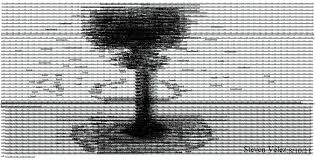
\includegraphics[width=.7\textwidth]{img/image_exercices/explosion.jpeg}
    \end{figure}
\end{frame}

\subsection{Solutions exercice 1}
\begin{frame}{Exercice 1: solutions}
    \centering
    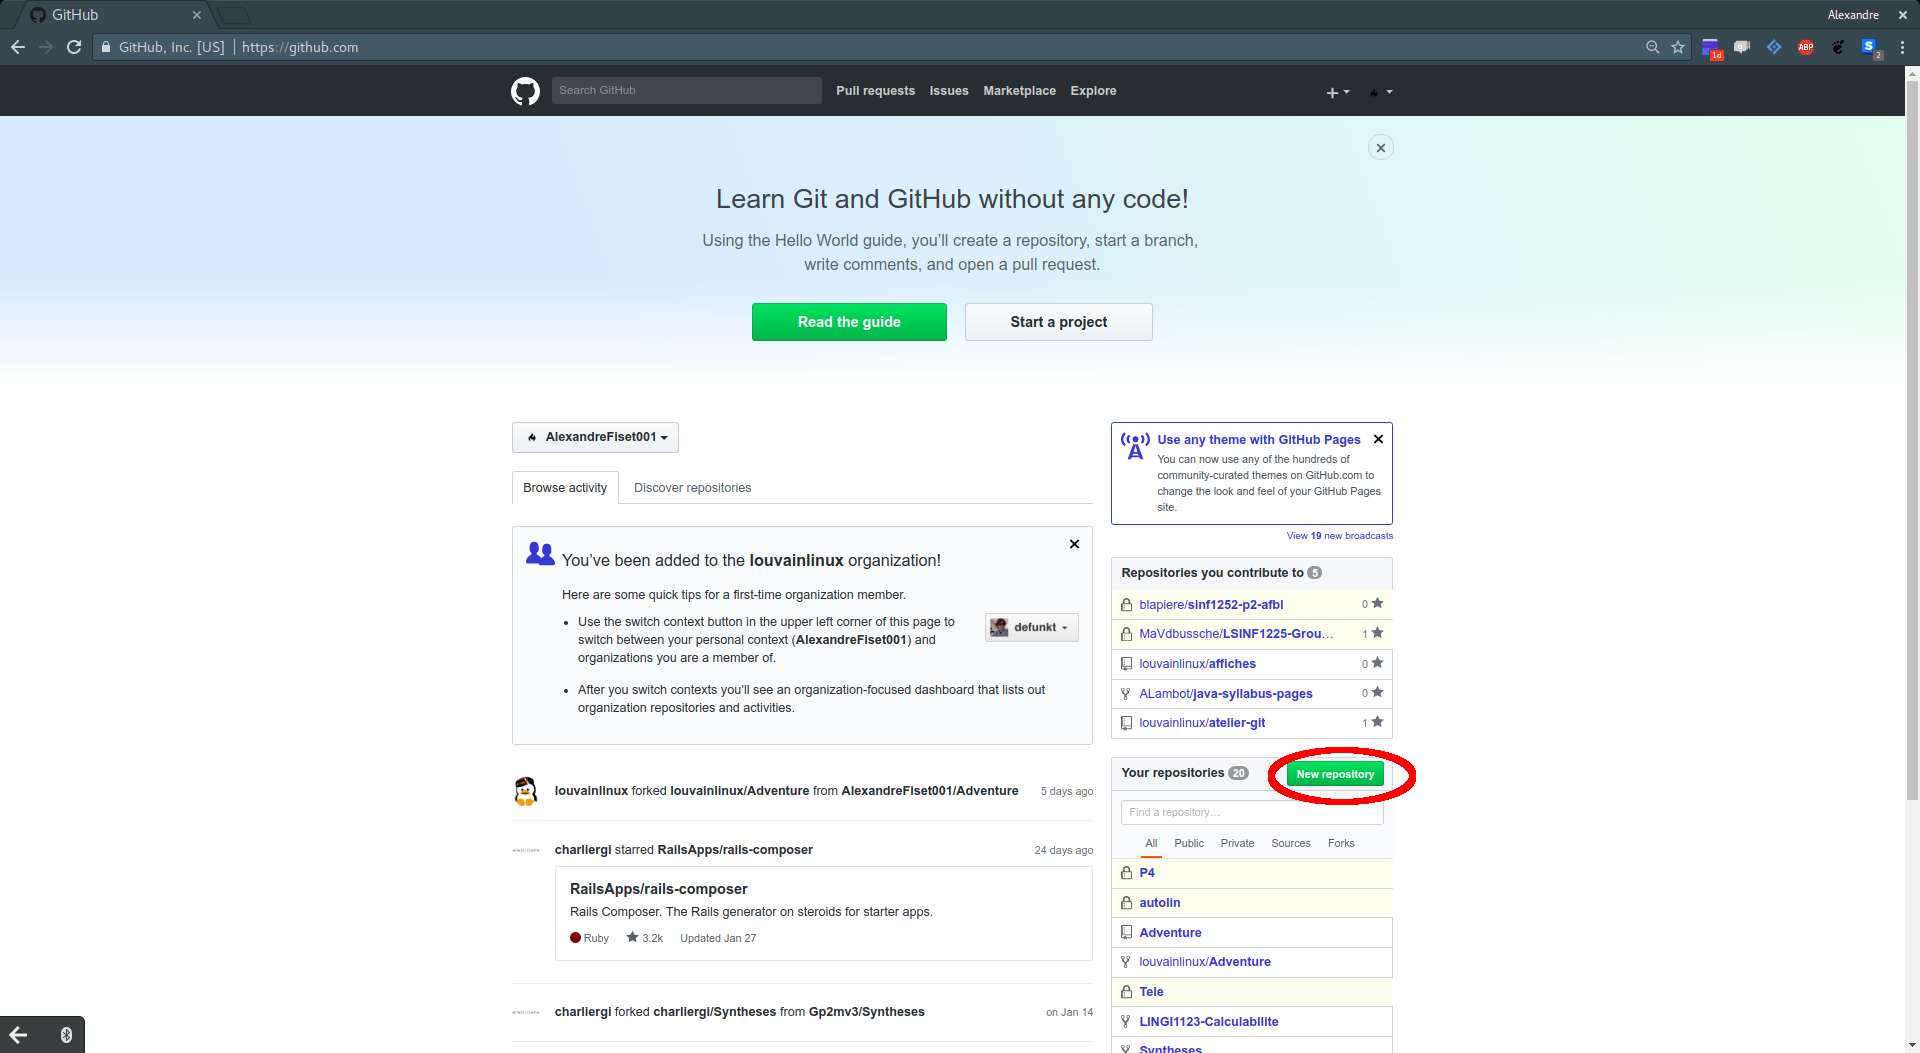
\includegraphics[width=\textwidth]{img/image_exercices/repo_creat.png}
\end{frame}

\begin{frame}{Exercice 1: solutions}
    \centering
    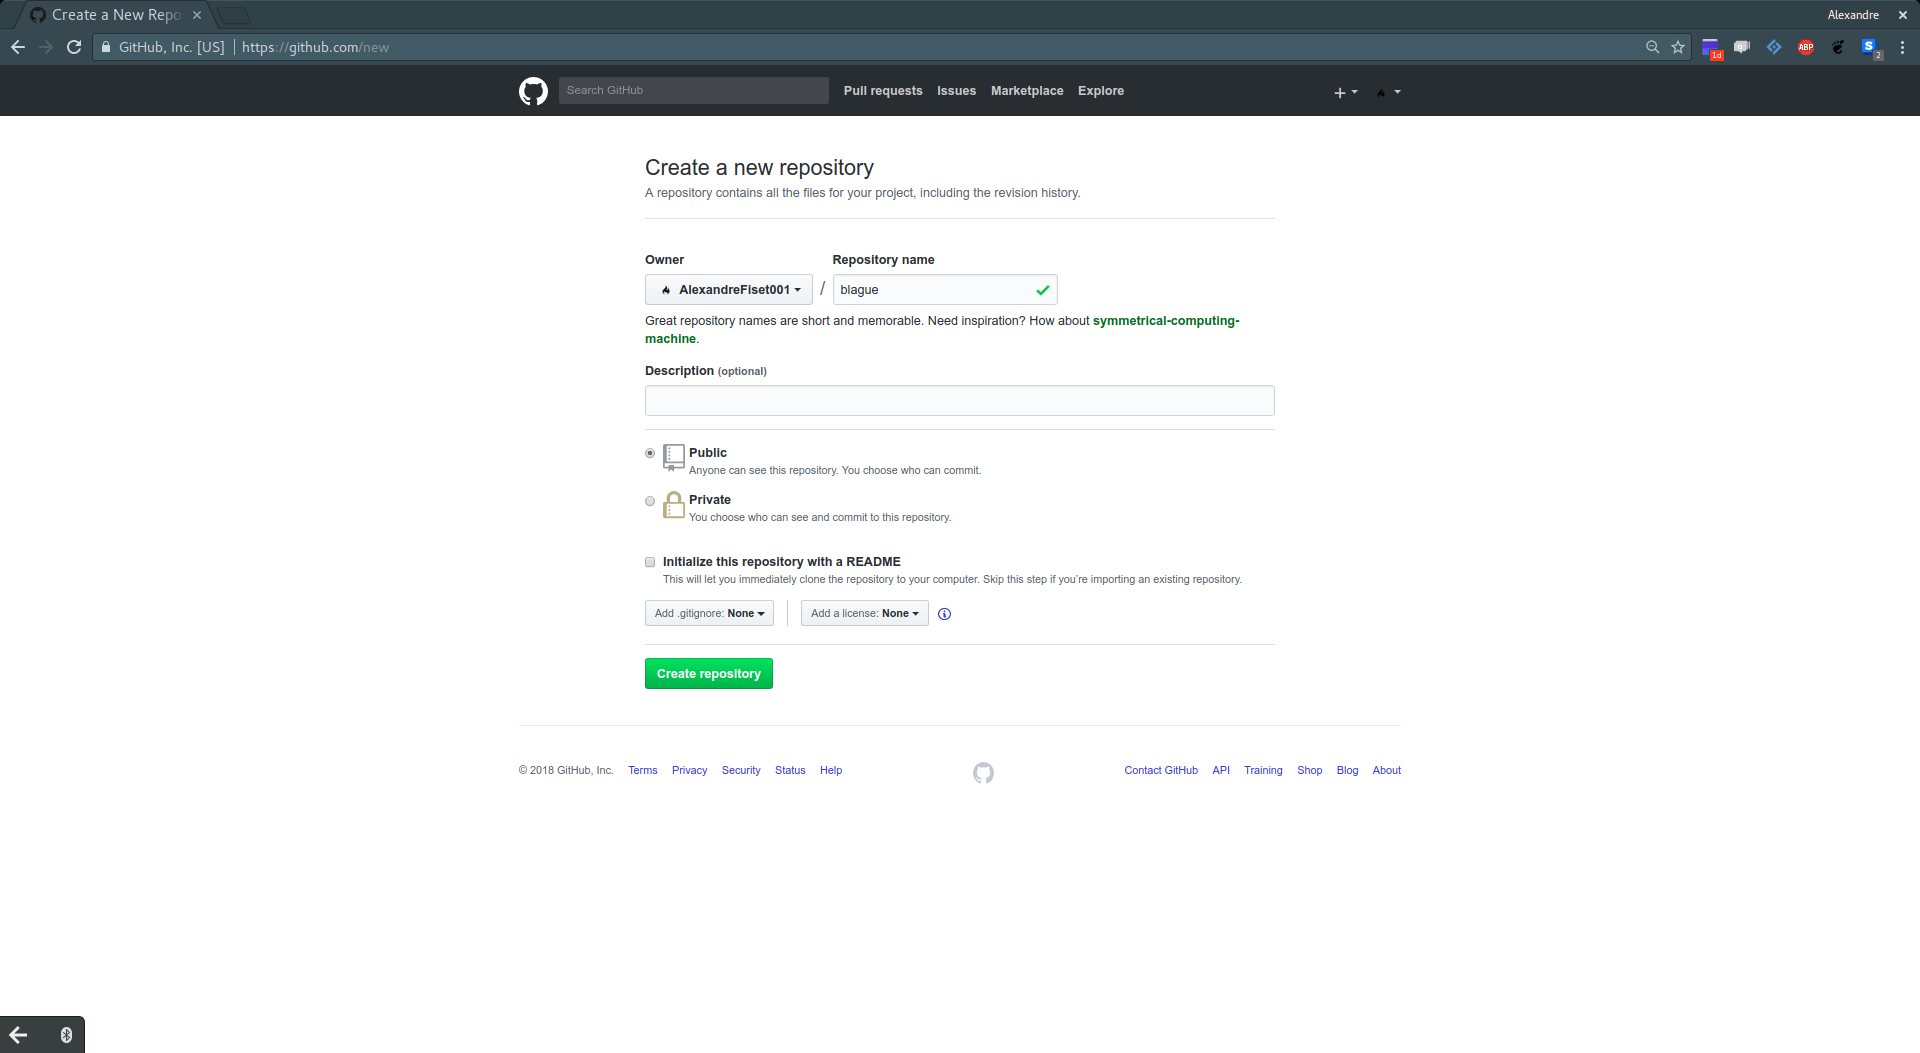
\includegraphics[width=\textwidth]{img/image_exercices/repo_config.png}
\end{frame}

\begin{frame}{Exercice 1: solutions}
    \centering
    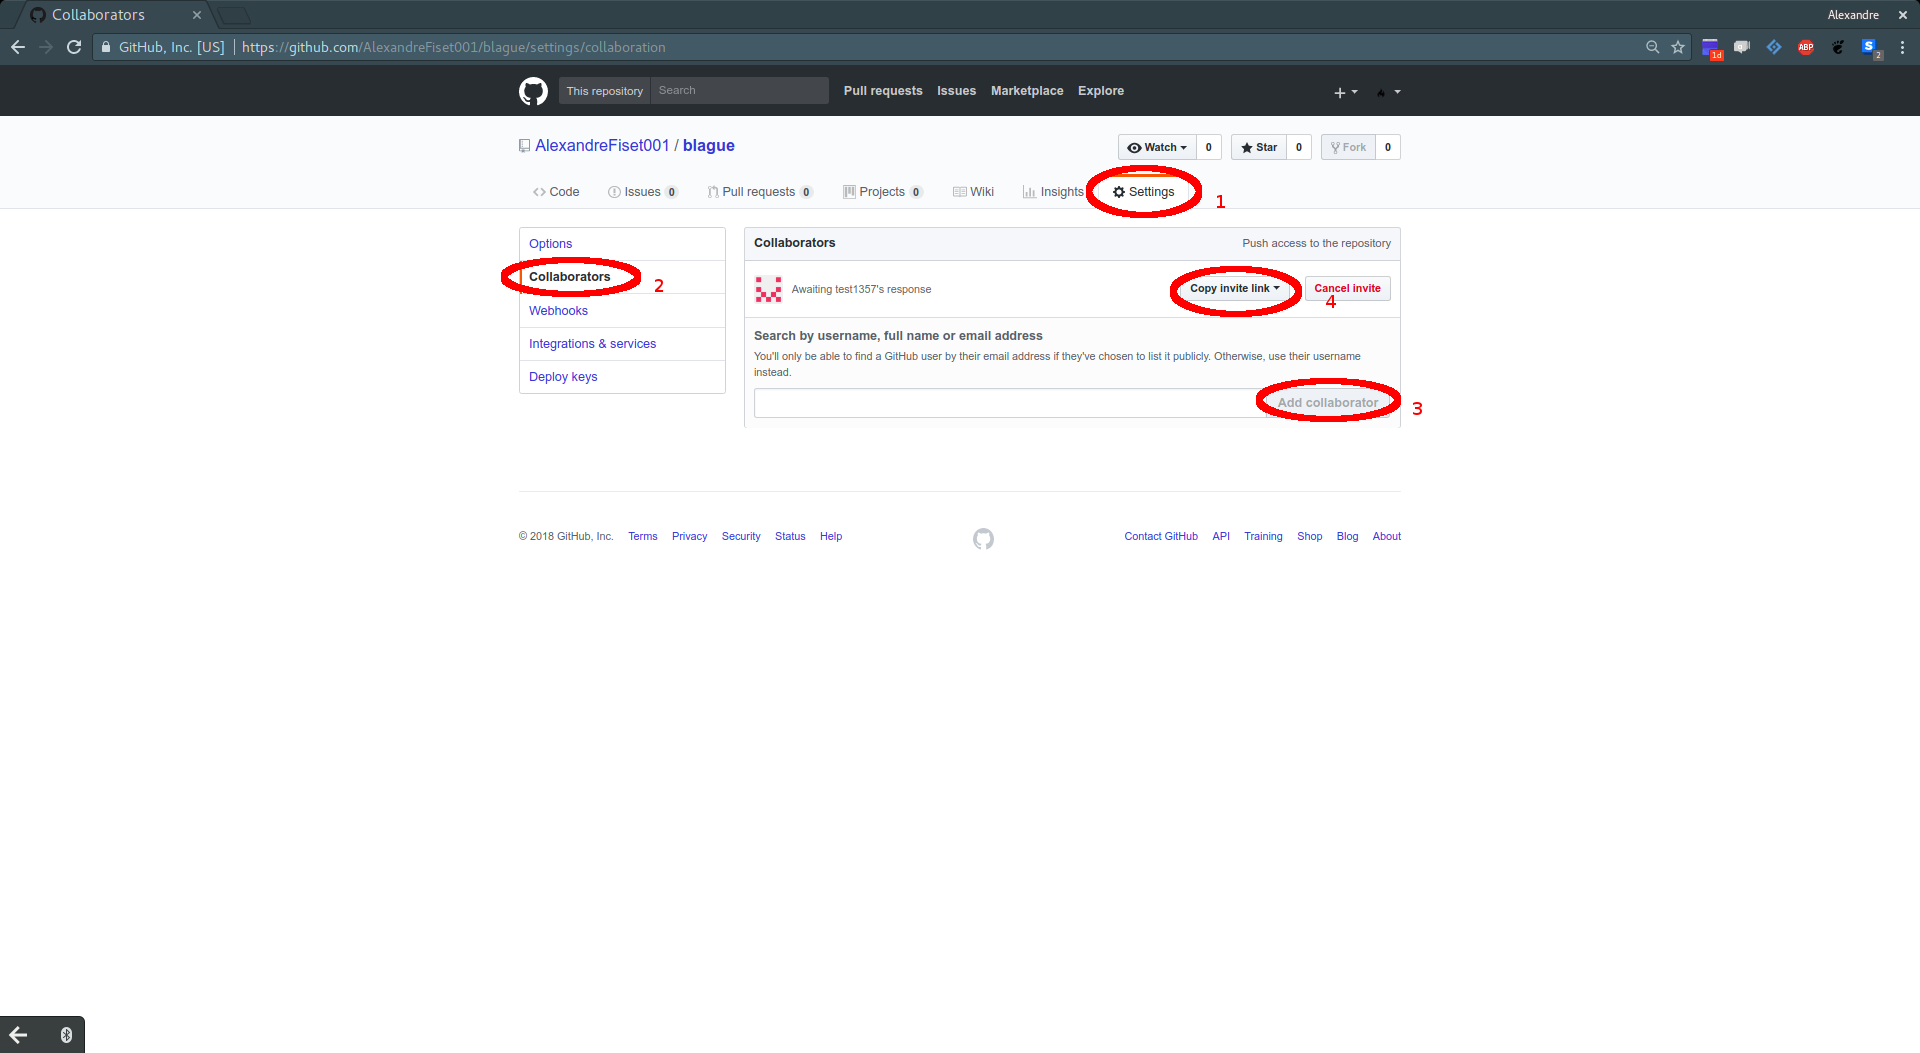
\includegraphics[width=\textwidth]{img/image_exercices/add_collab.png}
\end{frame}

\begin{frame}{Exercice 1: solutions}
    \centering
    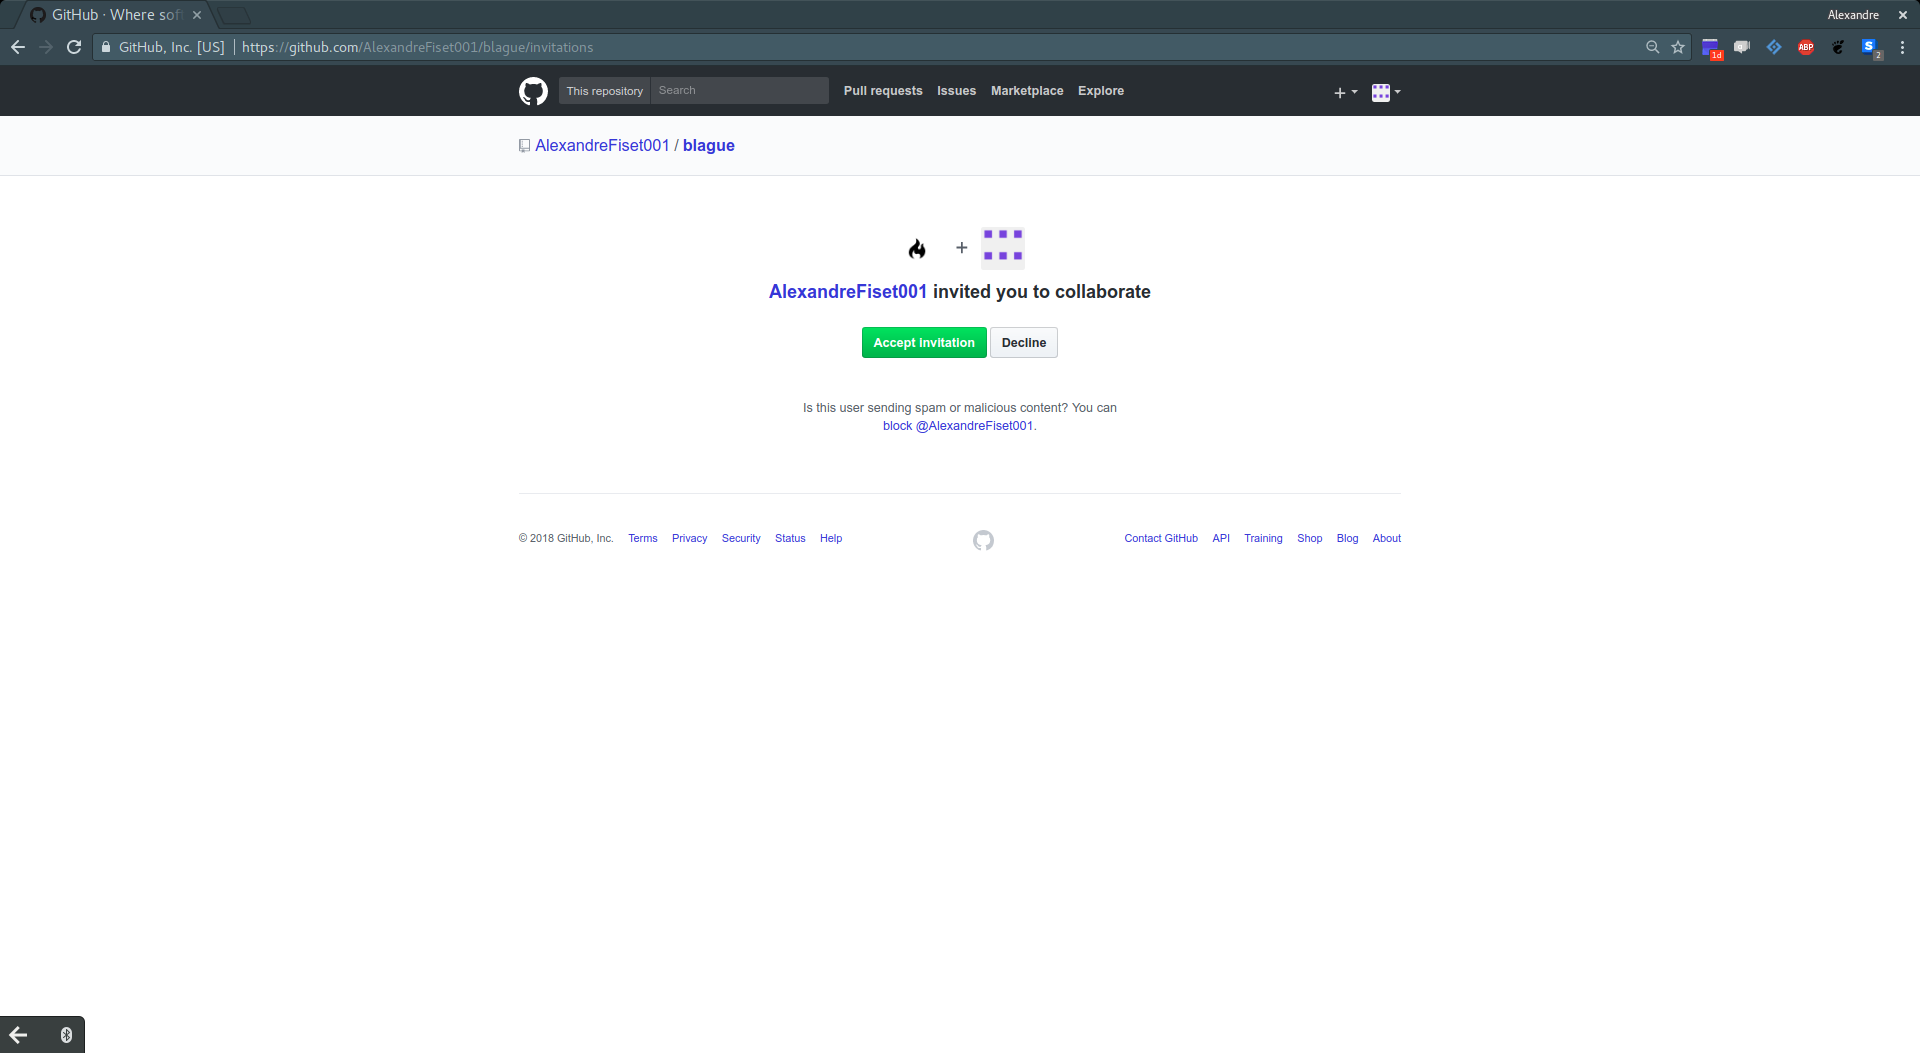
\includegraphics[width=\textwidth]{img/image_exercices/accept_invitation.png}
\end{frame}

\begin{frame}{Exercice 1: solutions}
    \centering
    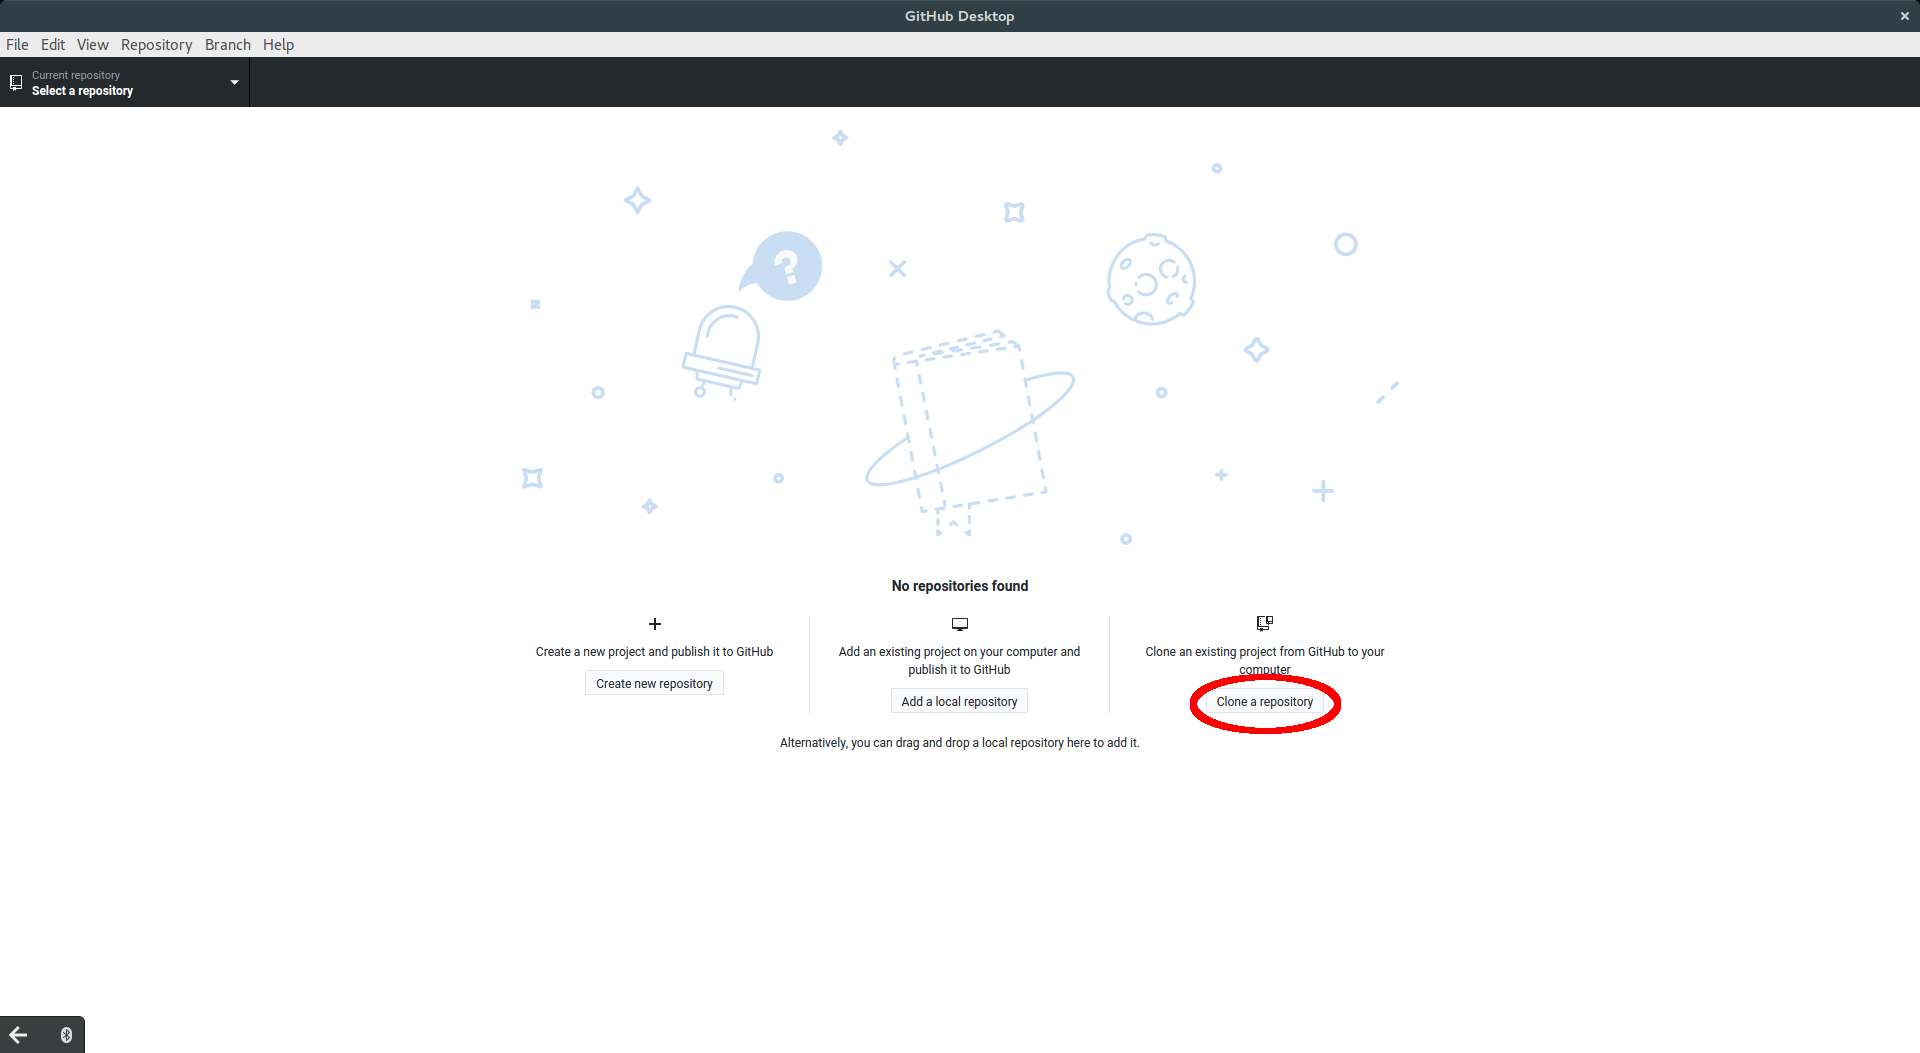
\includegraphics[width=\textwidth]{img/image_exercices/clonning_repo.png}
\end{frame}

\begin{frame}{Exercice 1: solutions}
    \centering
    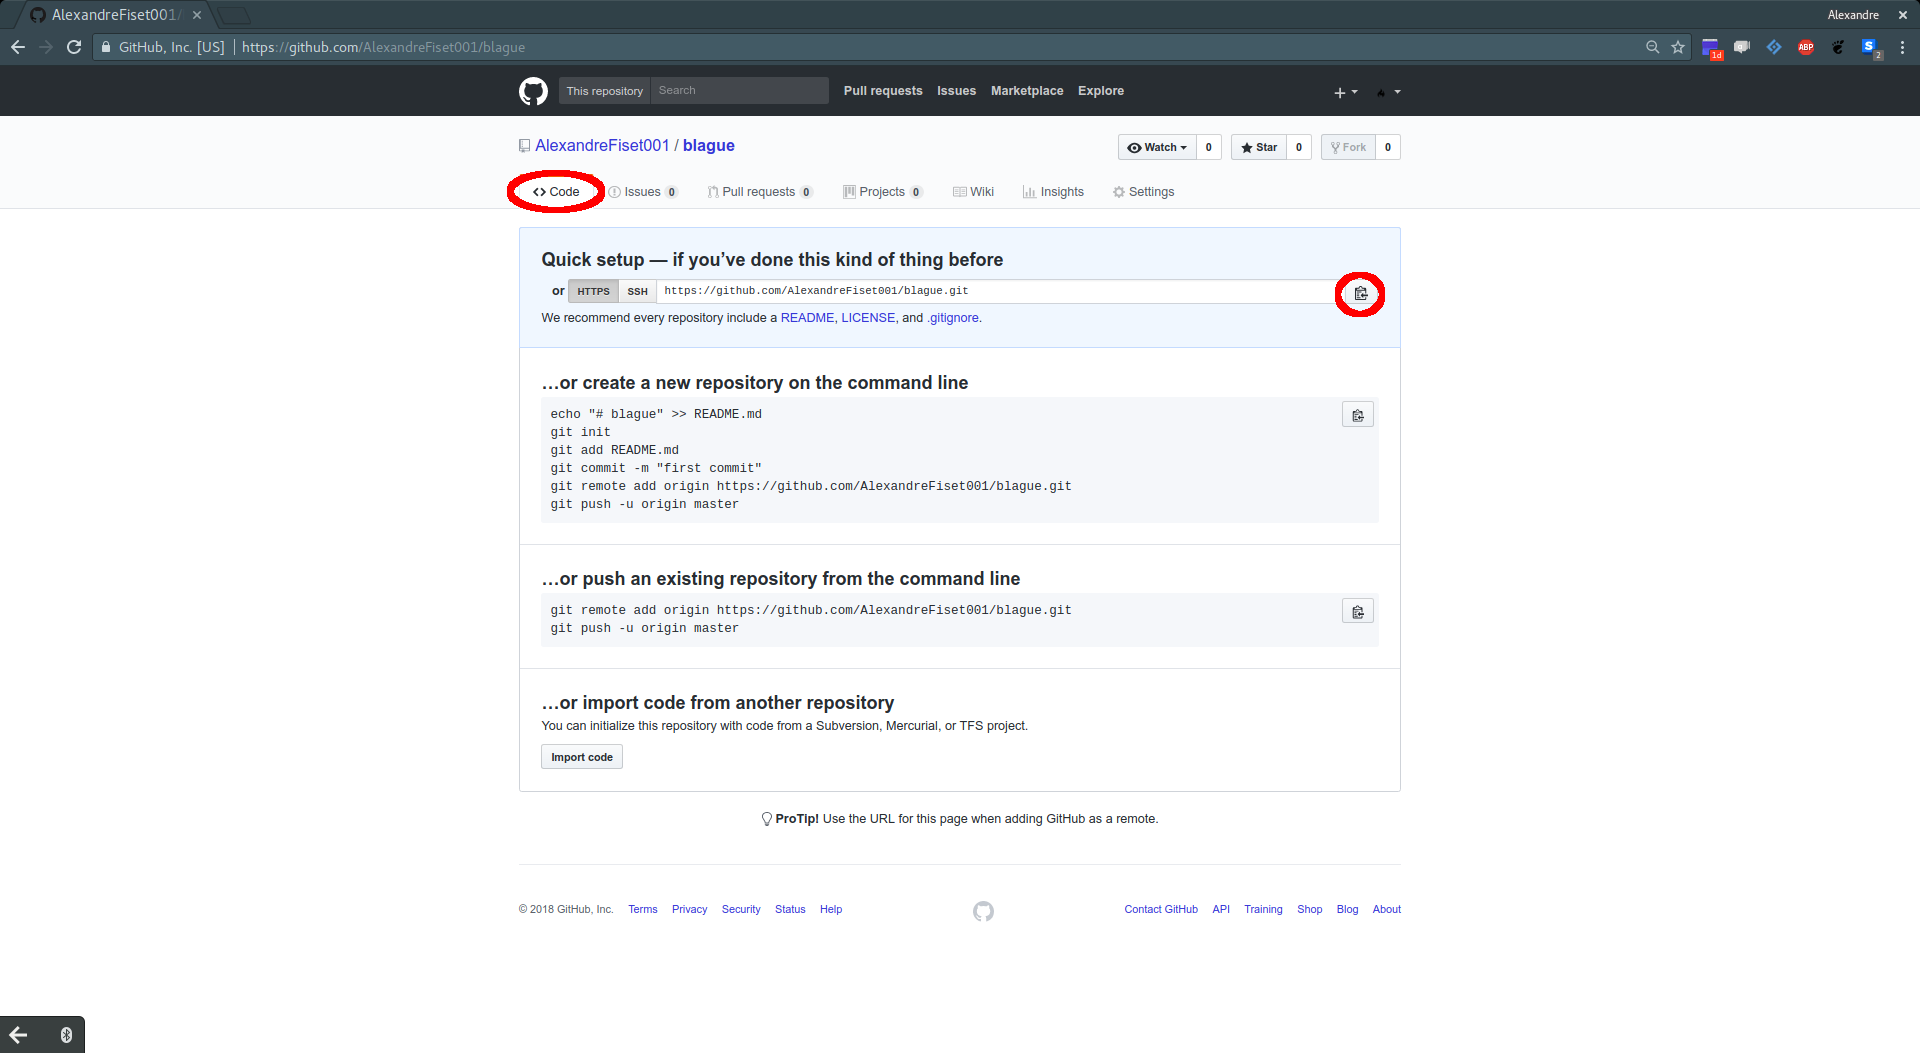
\includegraphics[width=\textwidth]{img/image_exercices/getting_url.png}
\end{frame}

\begin{frame}{Exercice 1: solutions}
    \centering
    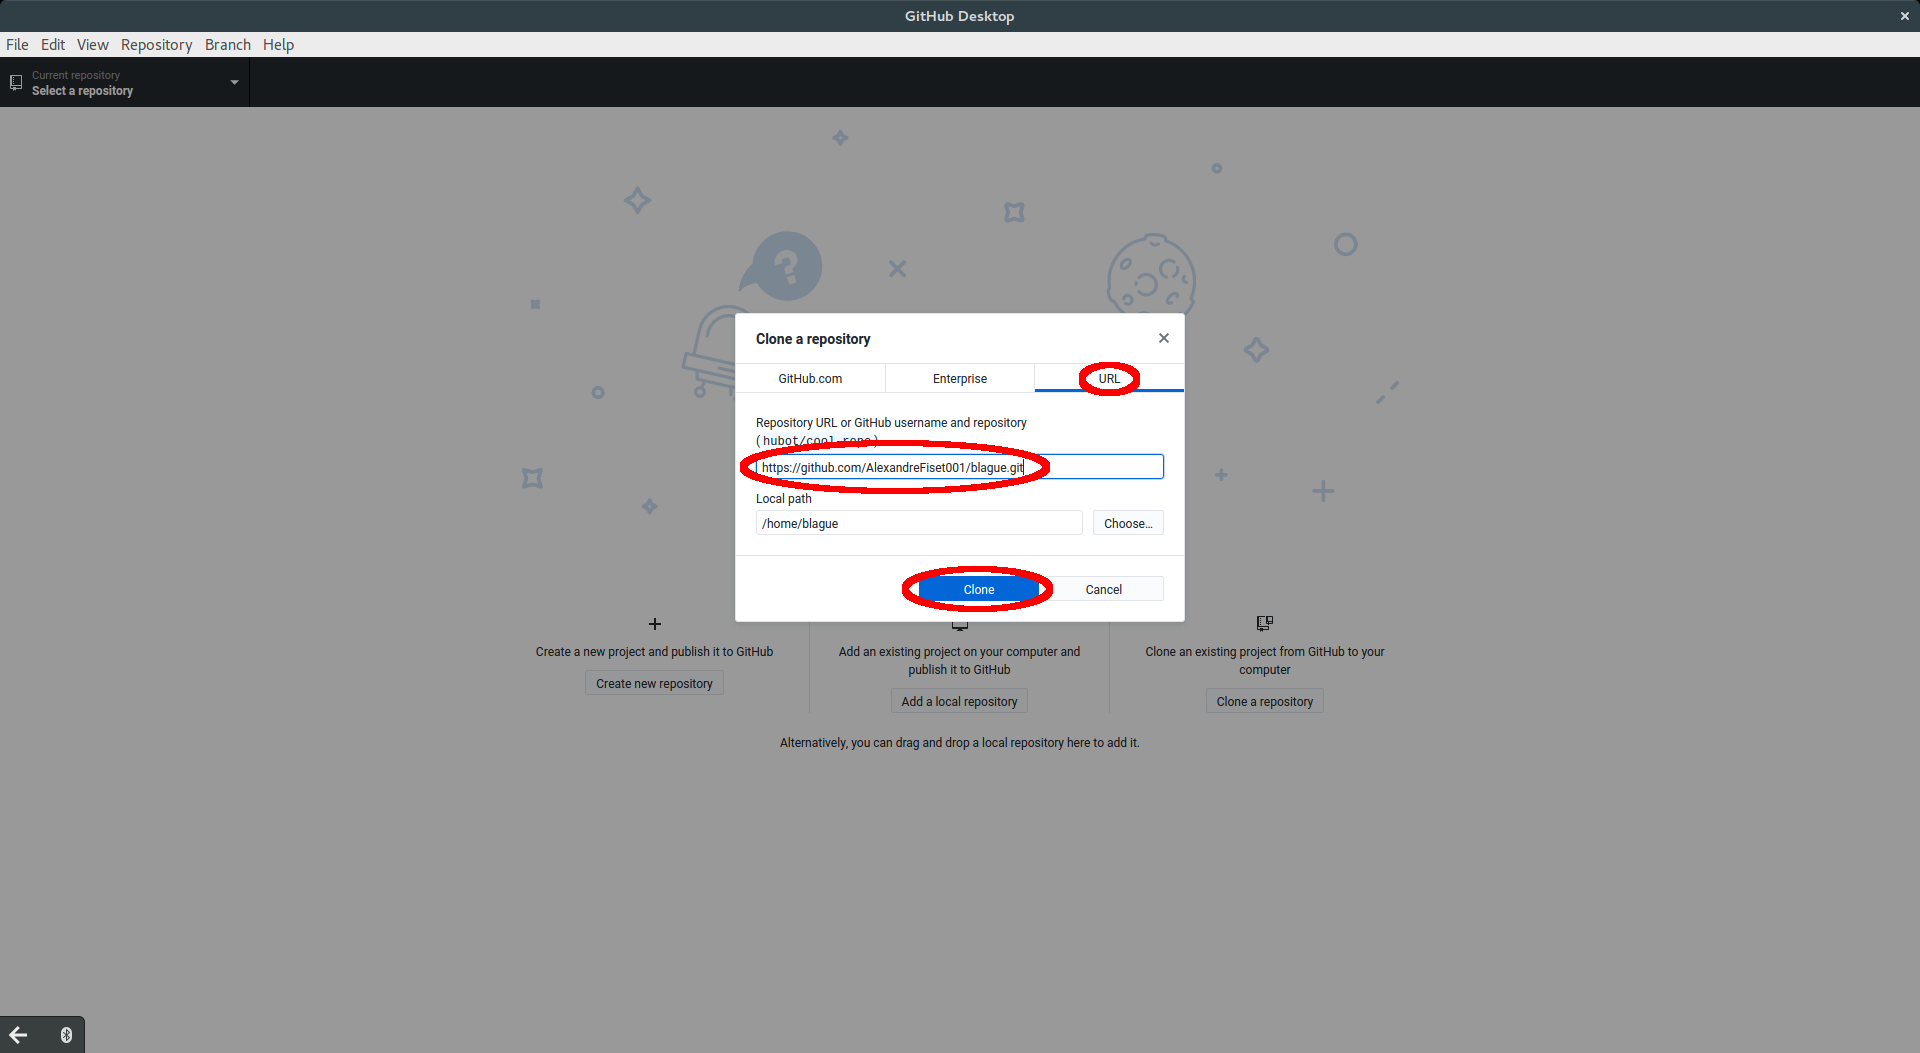
\includegraphics[width=\textwidth]{img/image_exercices/cloning_with_url.png}
\end{frame}

\begin{frame}{Exercice 1: solutions}
    \centering
    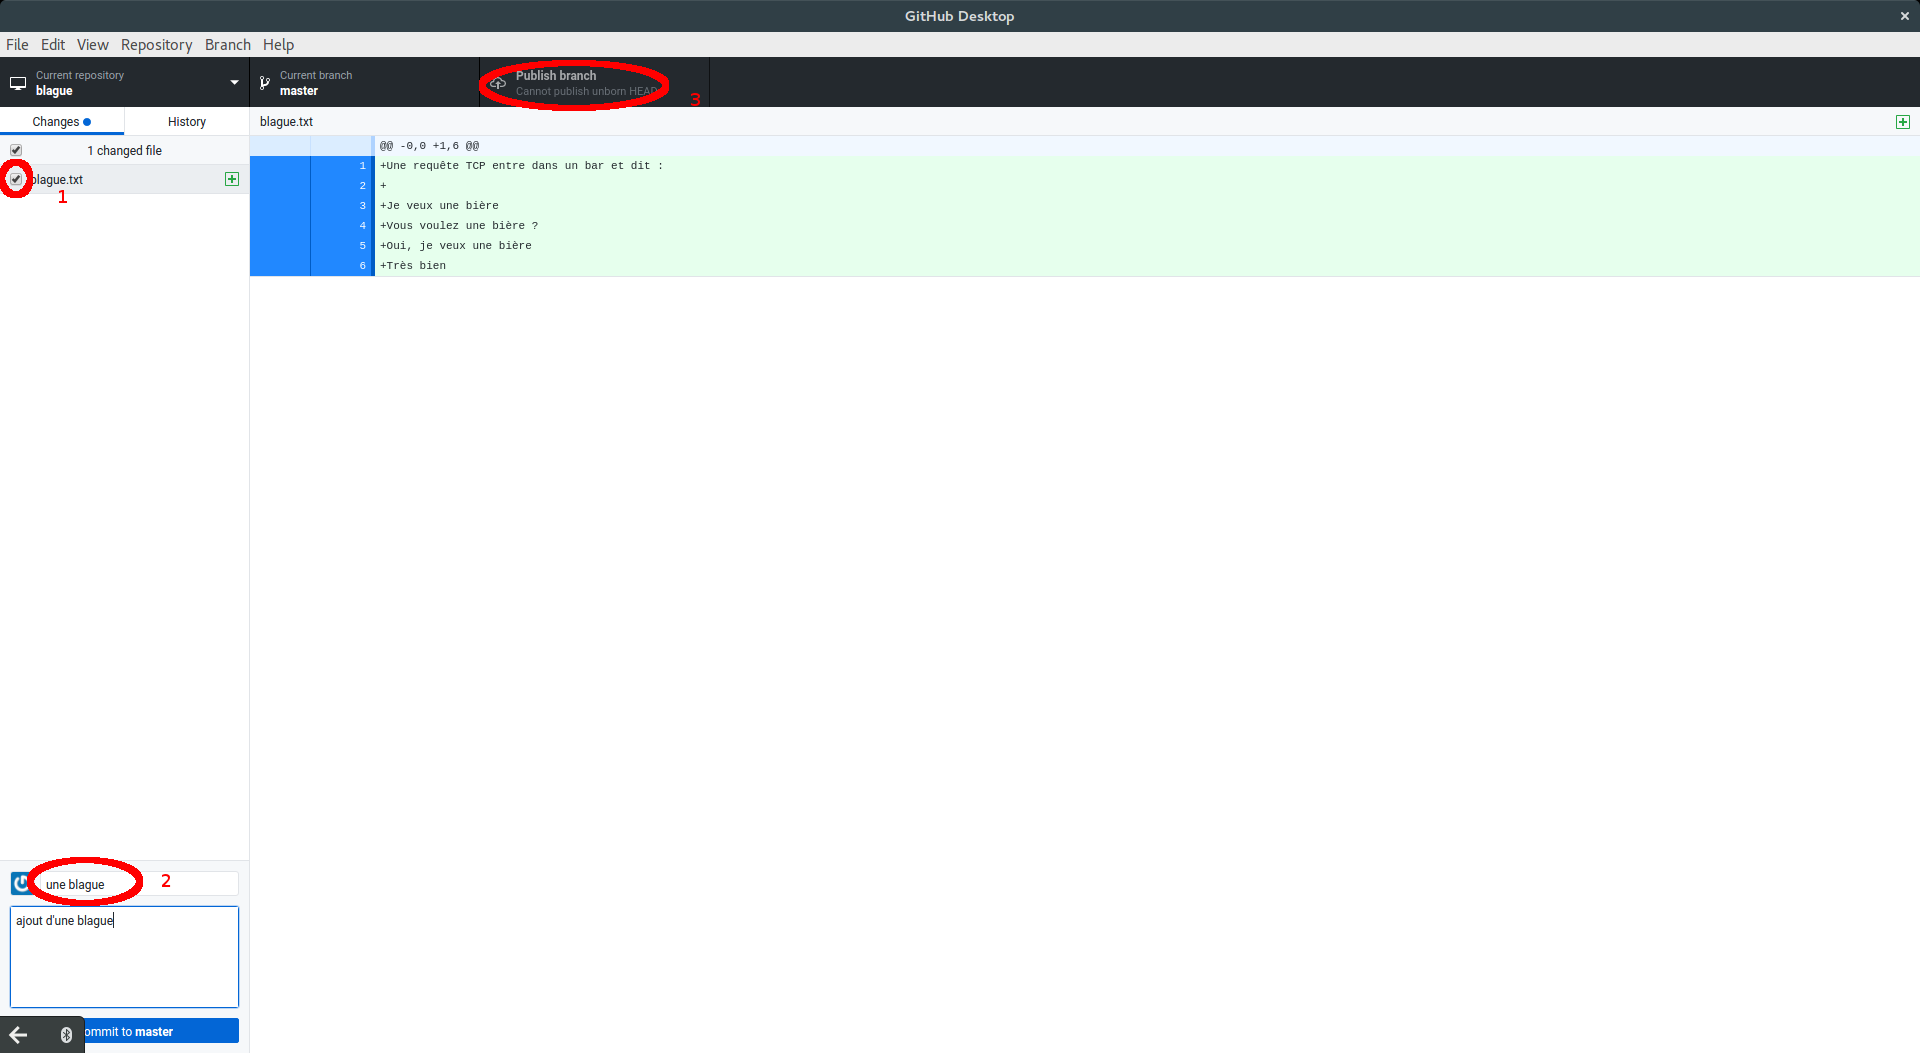
\includegraphics[width=\textwidth]{img/image_exercices/add+commit+push_1.png}
\end{frame}

\subsection{Solutions exercice 2}

\begin{frame}{Exercice 2 : solutions}
    \centering
    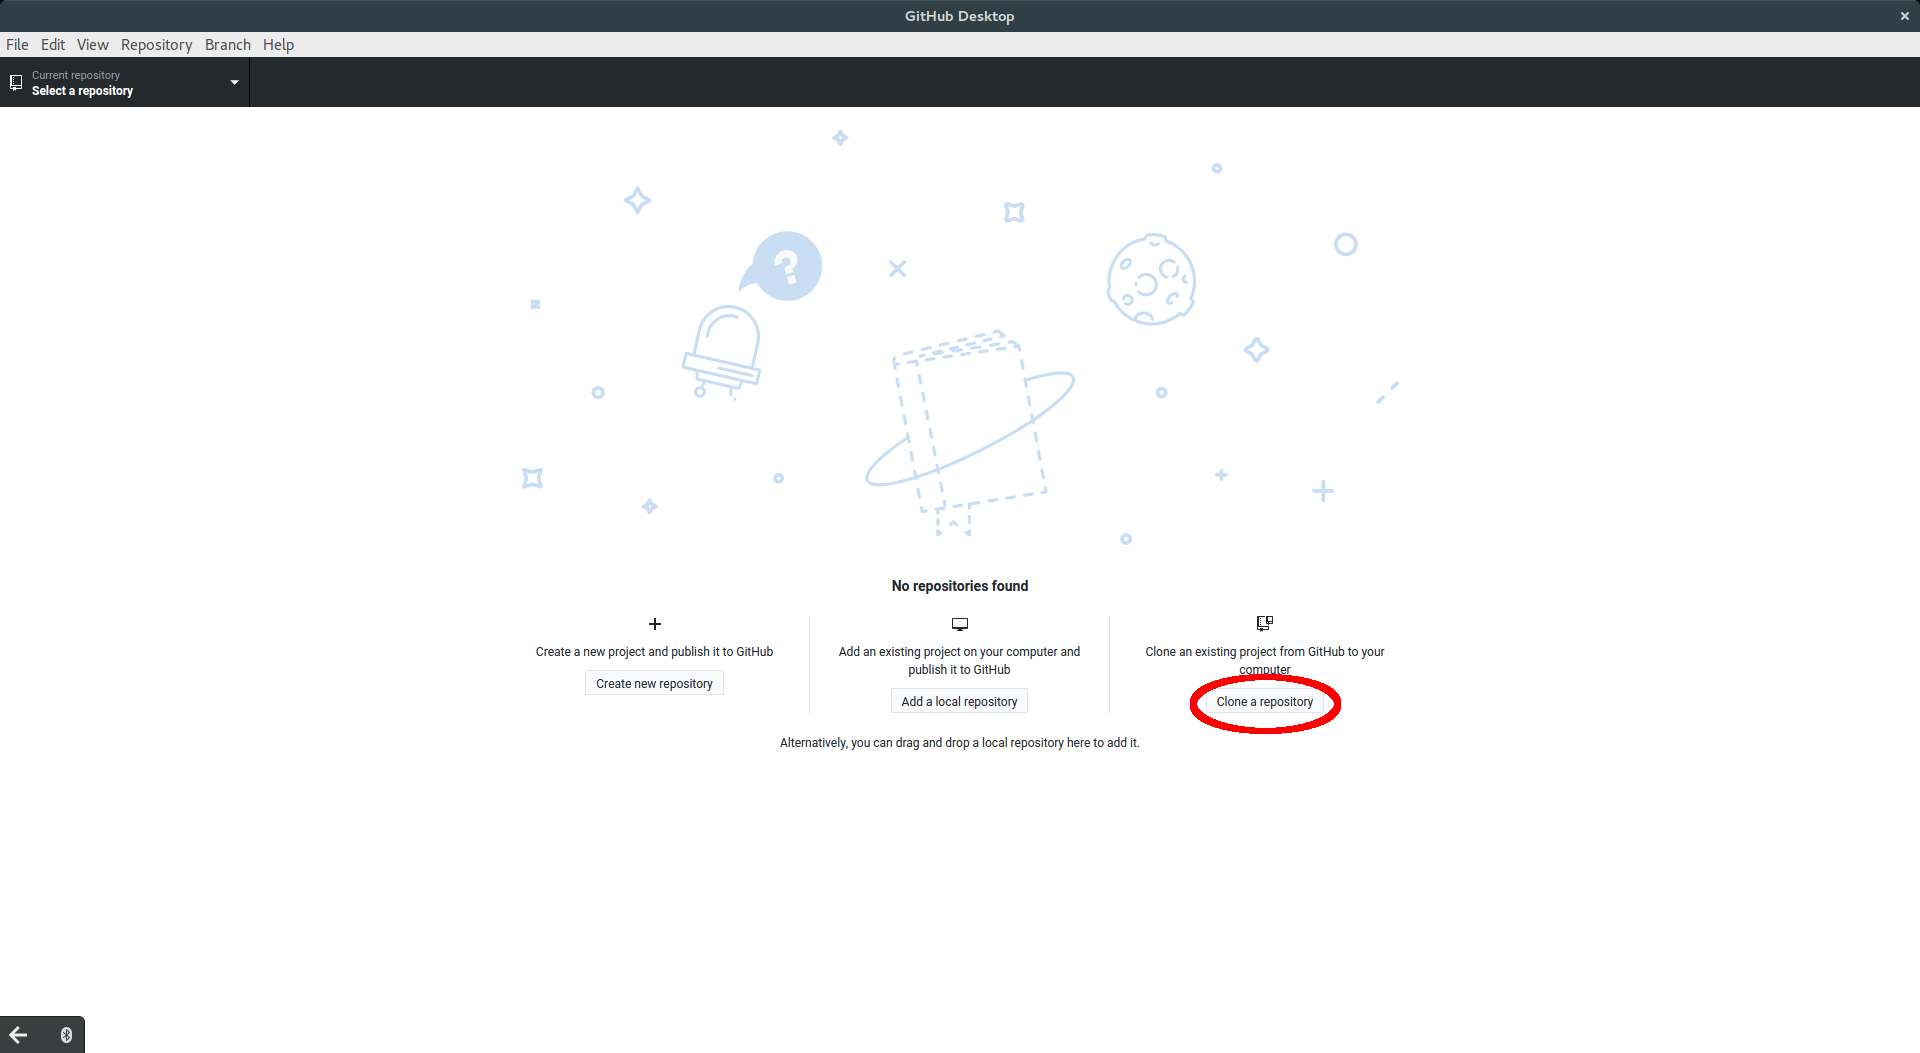
\includegraphics[width=\textwidth]{img/image_exercices/clonning_repo.png}
\end{frame}

\begin{frame}{Exercice 2: solutions}
	\centering
    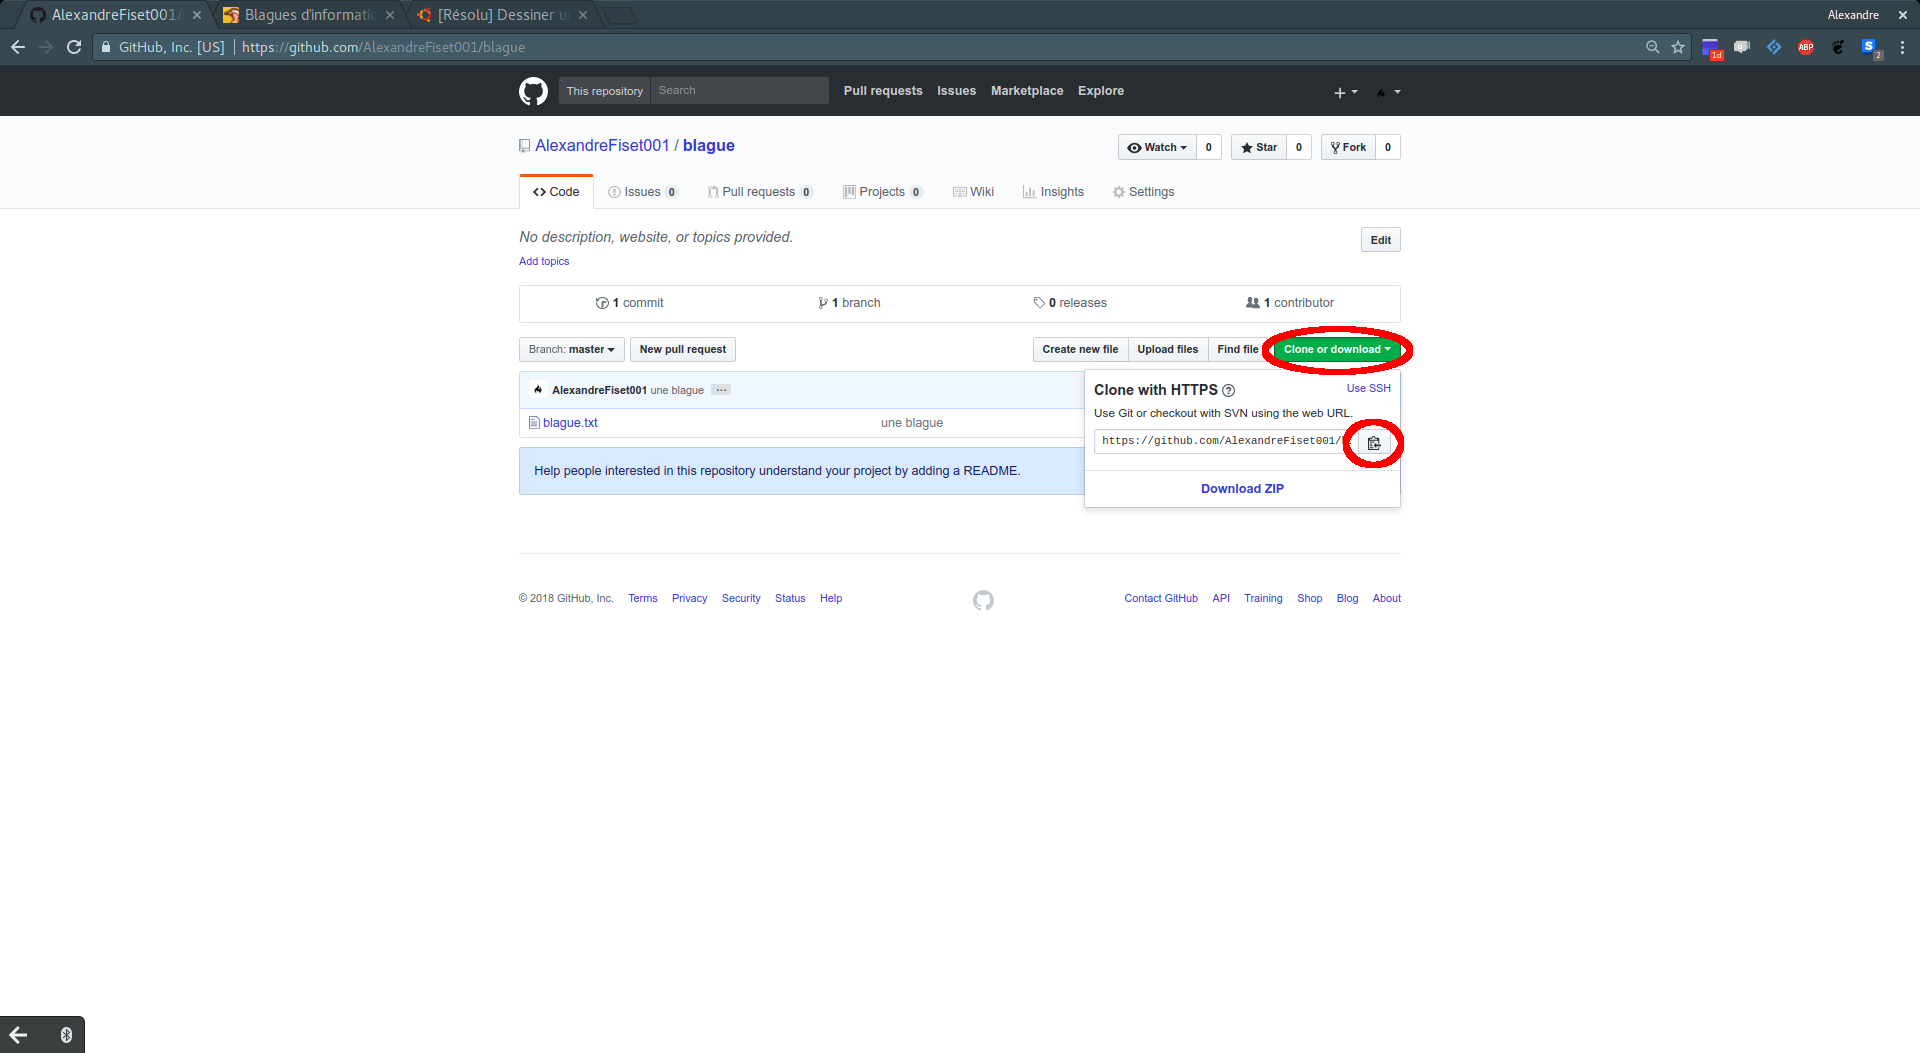
\includegraphics[width=\textwidth]{img/image_exercices/get_url_all_time.png}
\end{frame}

\begin{frame}{Exercice 2: solutions}
    \centering
    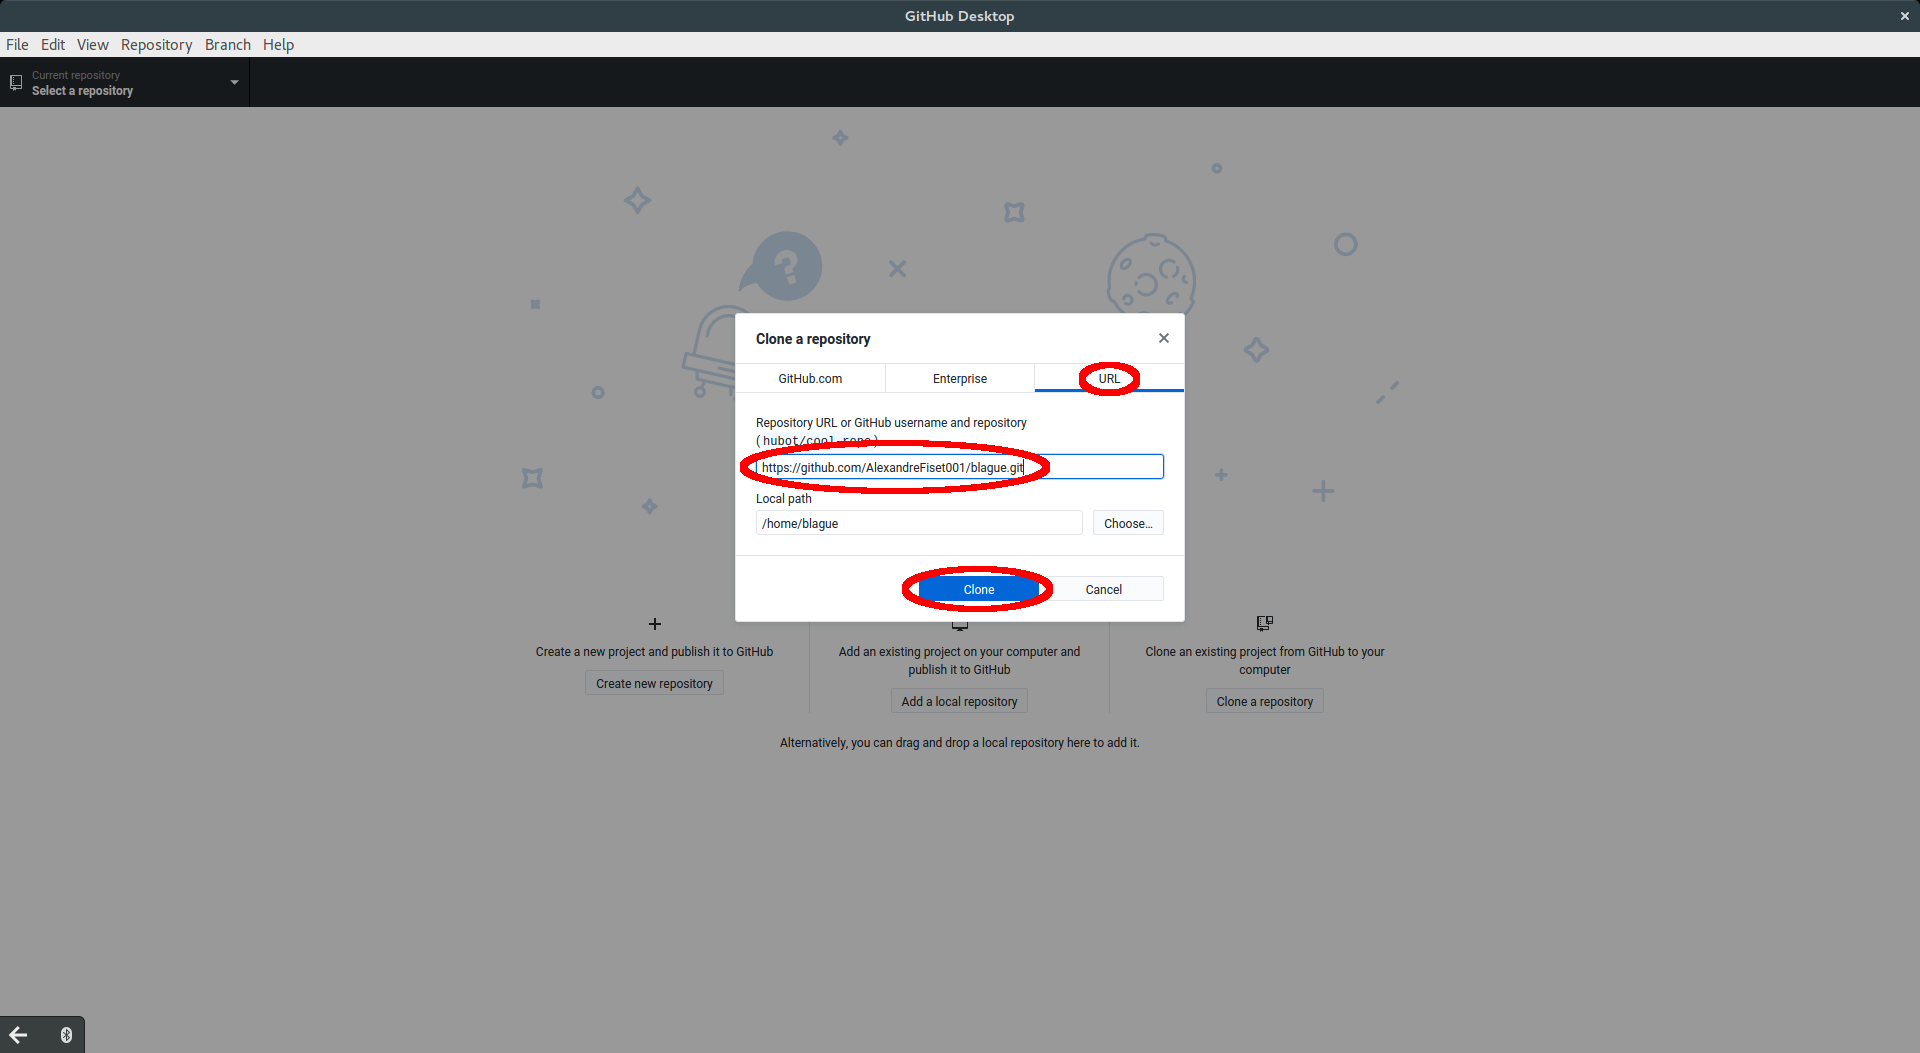
\includegraphics[width=\textwidth]{img/image_exercices/cloning_with_url.png}
\end{frame}

\begin{frame}{Exercice 2: solutions}
    \centering
    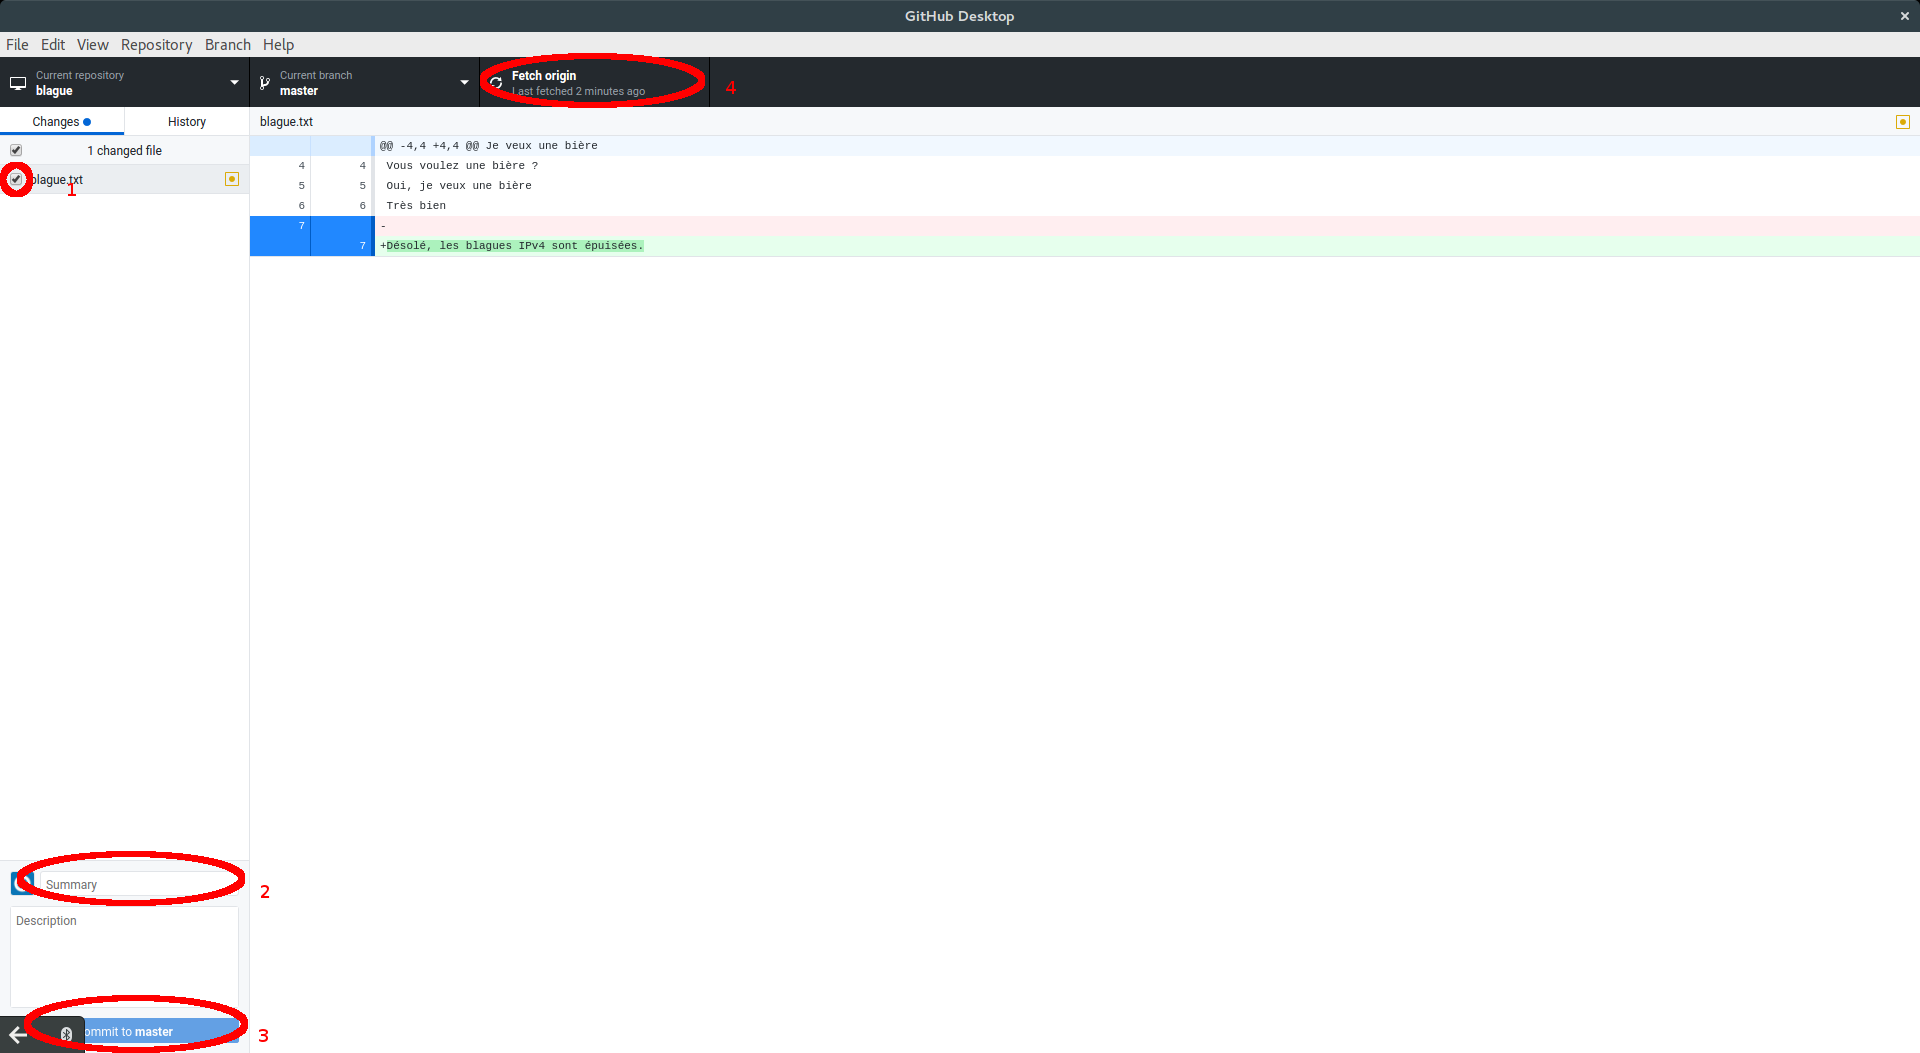
\includegraphics[width=\textwidth]{img/image_exercices/fetch_for_merge.png}
\end{frame}

\begin{frame}{Exercice 2: solutions}
    \centering
    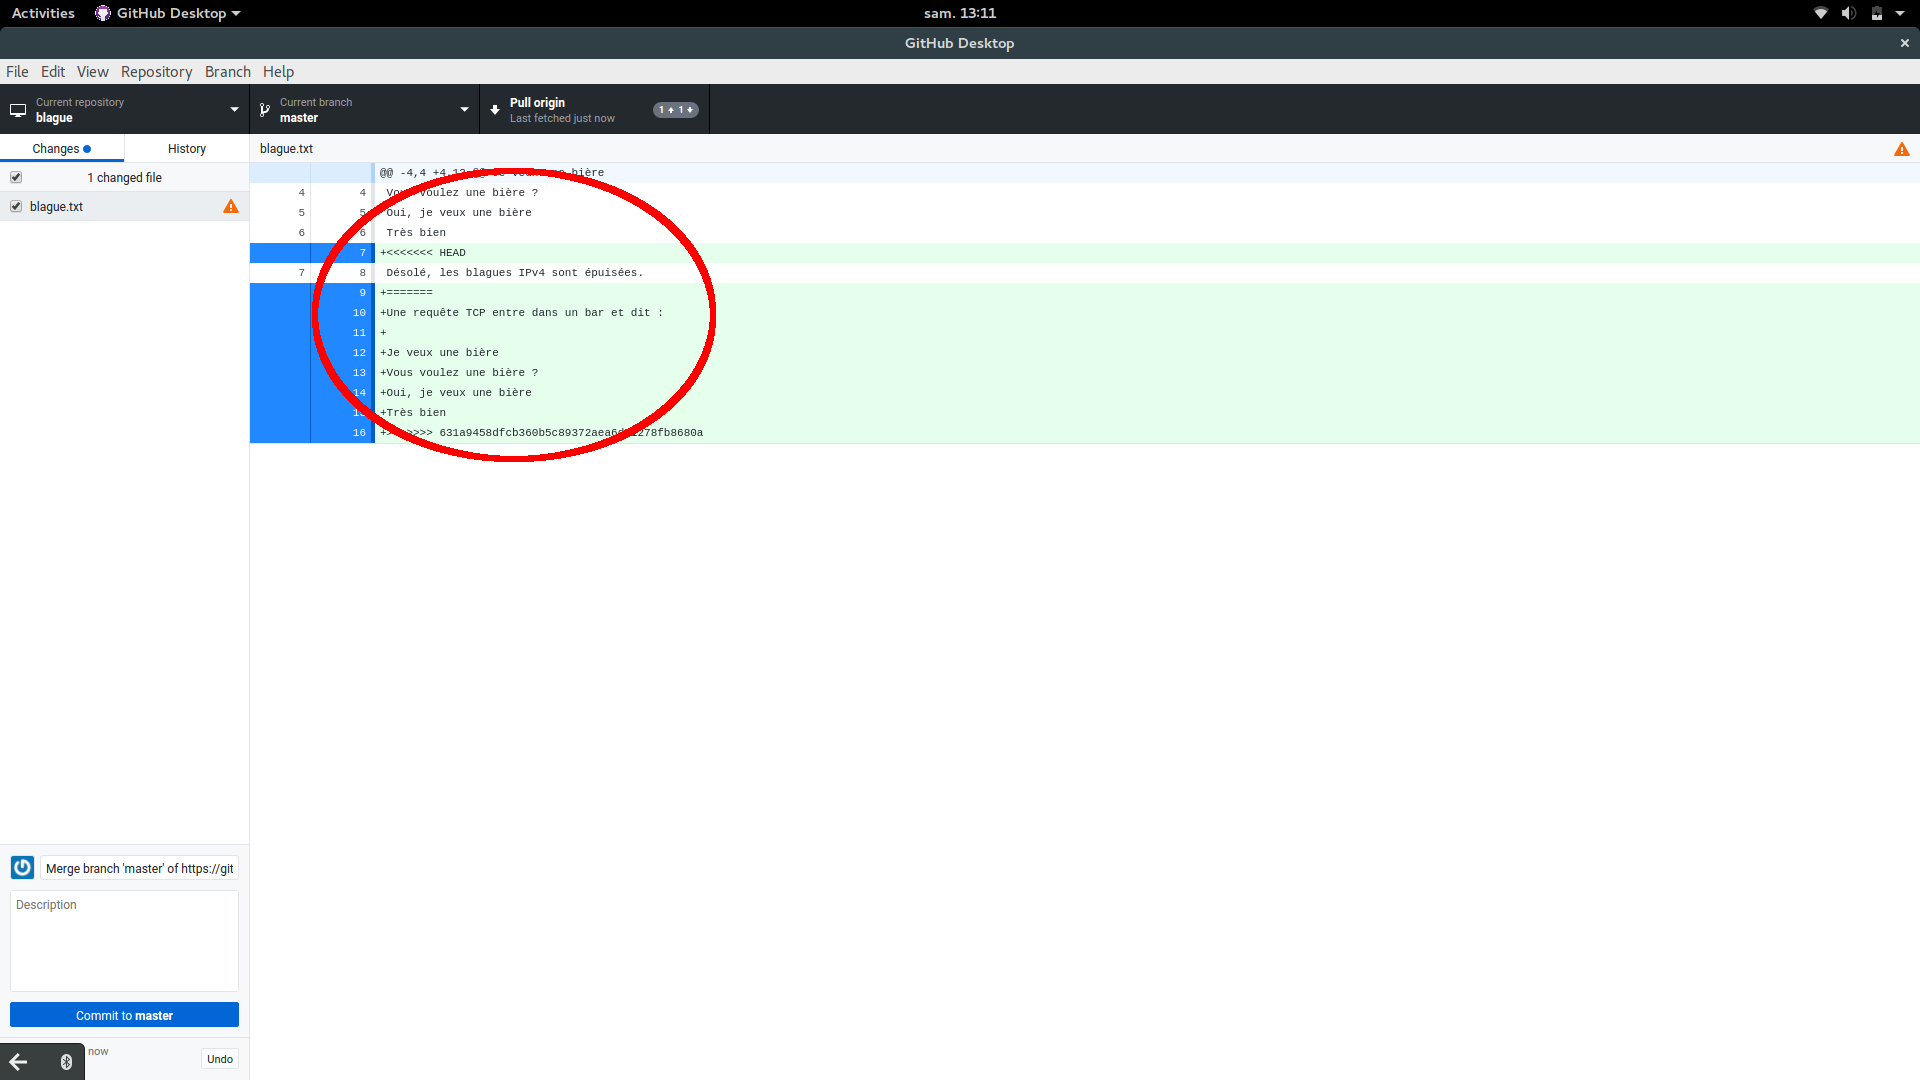
\includegraphics[width=\textwidth]{img/image_exercices/conflic_to_resolve.png}
\end{frame}

\begin{frame}{Exercice 2: solutions}
	\centering
    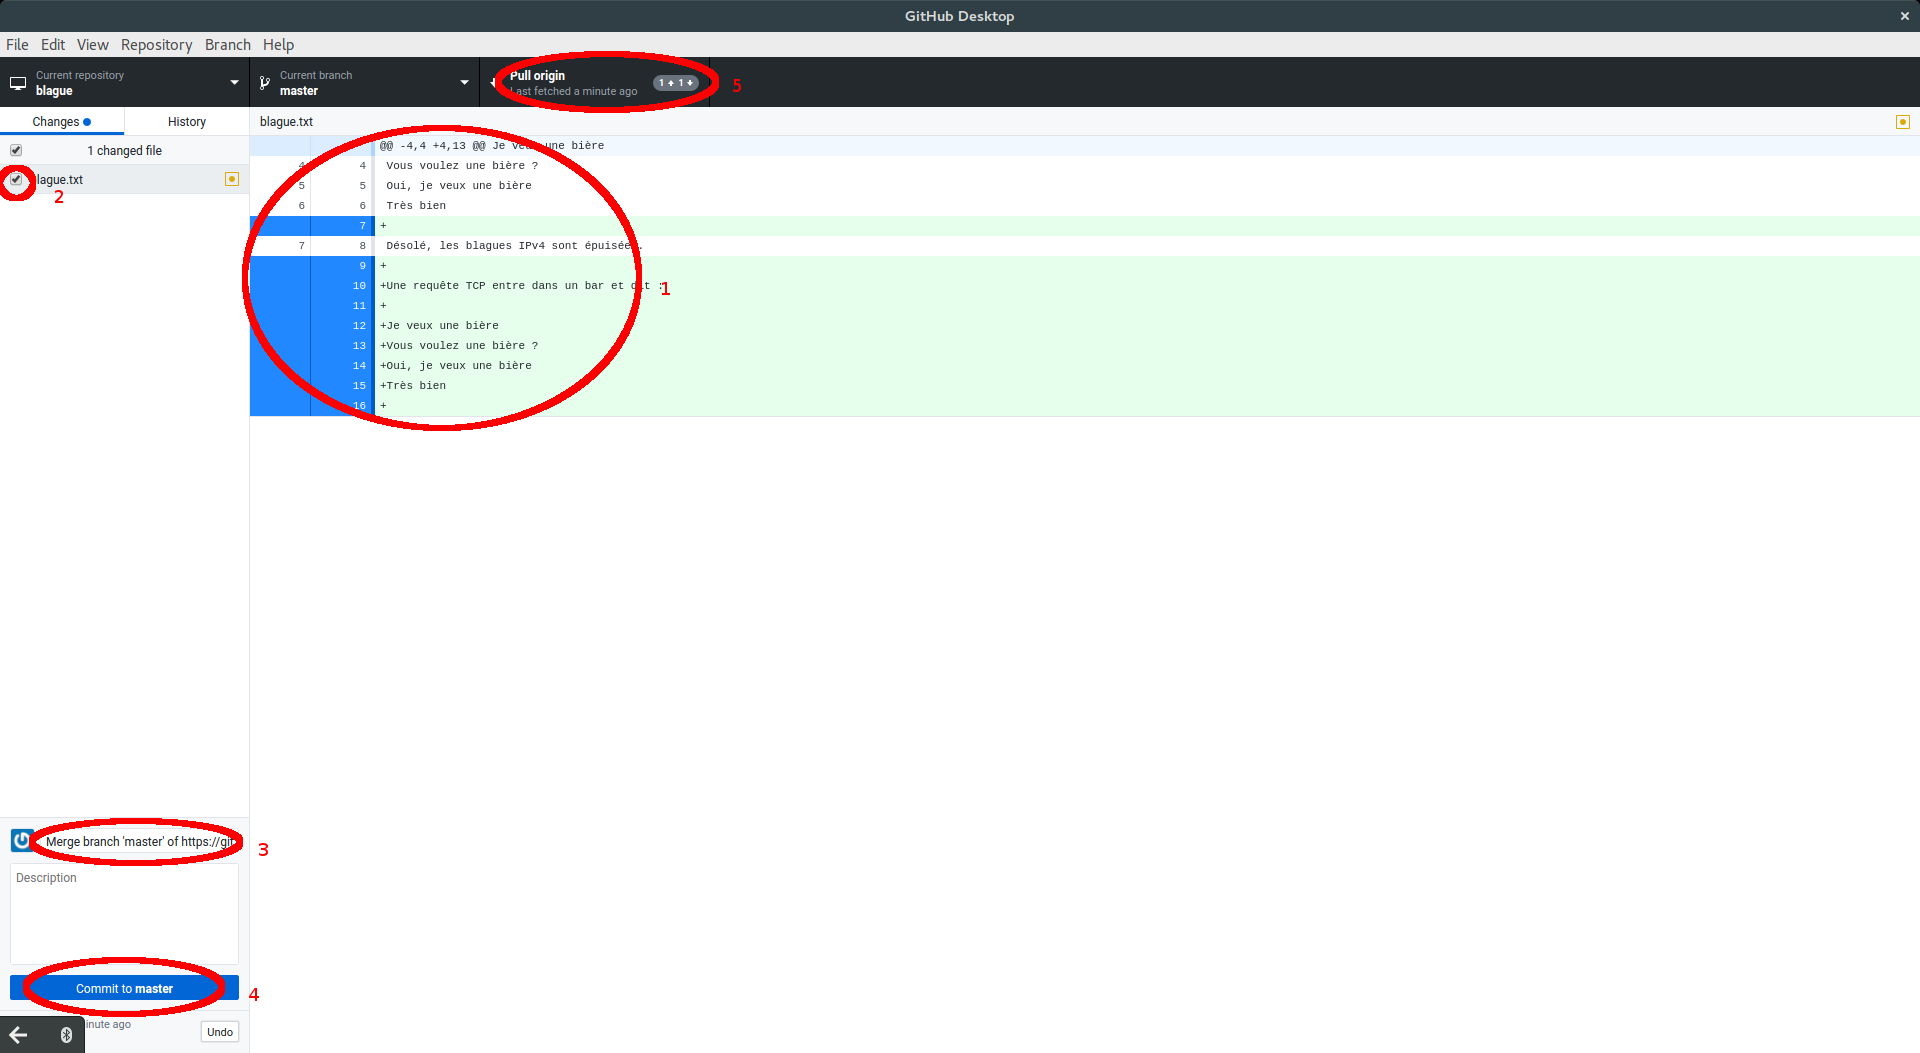
\includegraphics[width=\textwidth]{img/image_exercices/conflic_resolv.png}
\end{frame}

\begin{frame}{Exercice 2: solutions}
    Après le merge, l'historique observé dans GitHub Desktop peut ne pas être
    le même chez les différentes personnes.
    Cela est dû au fait que GitHub Desktop n'affiche pas l'entièreté de
    l'historique, mais seulement les commits qu'il juge pertinents.

    Pour voir tout l'historique, aller sur le site \url{github.com} ou bien
    utiliser une autre interface de git (ex.: commande \texttt{git log}).
\end{frame}

\subsection{Solutions exercice 3}

\begin{frame}{Exercice 3: solutions}
    Cette solution est presque identique à la solution de l'exercice 1, sauf
    qu'il est impossible de faire le merge avec GitHub Desktop. Il faut
    utiliser une autre interface de git (voir plus loin dans les slides).
\end{frame}

\section{Fonctionnalités plus avancées}

\subsection{Les branches}

\begin{frame}{De derrière: les objets git}
    \begin{itemize}
        \item Chaque commit a un identifiant: \textbf{12f87}b95caff8cbeb5ce0717528d77e27db5669c.
    \end{itemize}
    \begin{center}
    \includegraphics[width=0.8\textwidth]{img/commit-and-tree.png}
    \end{center}
\end{frame}

\begin{frame}{De derrière: les parents}
    \begin{itemize}
        \item Chaque commit a un parent.
    \end{itemize}
    \includegraphics[width=\textwidth]{img/commits-and-parents.png}
\end{frame}

\begin{frame}{Récupérer un fichier d'un commit passé}
    \begin{center}
    	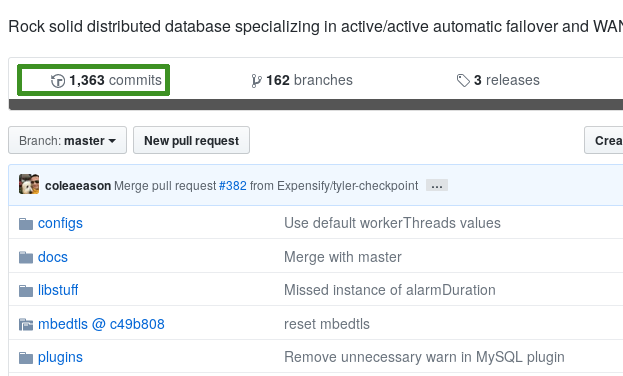
\includegraphics[scale=0.5]{img/rollback_1.png}
    \end{center}
\end{frame}

\begin{frame}{Récupérer un fichier d'un commit passé}
    \begin{center}
    	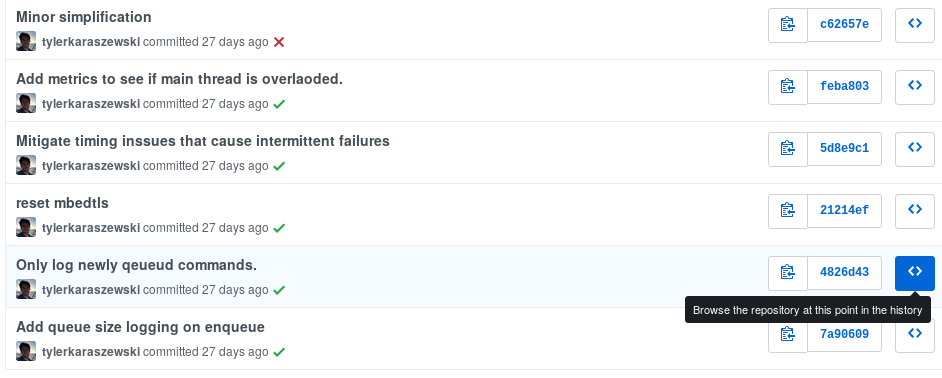
\includegraphics[scale=0.3]{img/rollback_2.png}
    \end{center}
\end{frame}

\begin{frame}{Récupérer un fichier d'un commit passé}
    \begin{center}
    	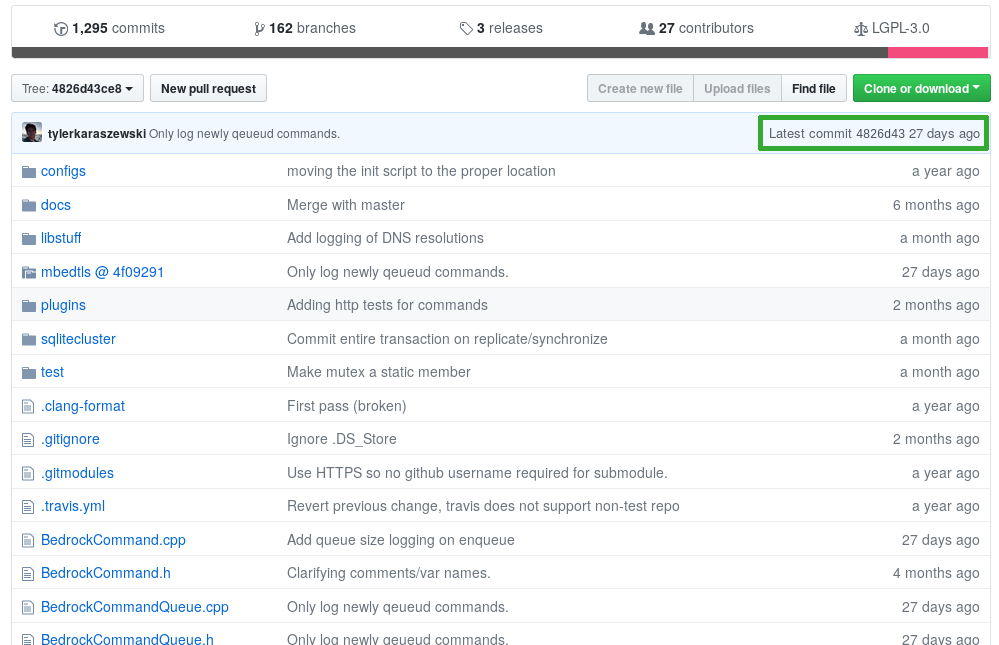
\includegraphics[scale=0.3]{img/rollback_3.png}
    \end{center}
\end{frame}

\begin{frame}{De derrière: les étiquettes}
    \begin{itemize}
        \item On peut mettre des étiquettes sur des commits.
        \item \texttt{HEAD} est la position actuelle.
    \end{itemize}
    \includegraphics[width=\textwidth]{img/branch-and-history.png}
\end{frame}

\begin{frame}{Créer une branche}
    \begin{itemize}
        \item Une branche est une nouvelle étiquette.
        \item La branche par défaut est \texttt{master}.
    \end{itemize}
    \begin{center}
        \includegraphics[width=0.8\textwidth]{img/head-to-master.png}
    \end{center}
\end{frame}

\begin{frame}{Changer de branche}
    La branche courante est celle qui suit les nouveaux commits.
    \begin{columns}
        \begin{column}{0.44\textwidth}
            \begin{center}
                \includegraphics[width=\textwidth]{img/head-to-testing.png}
            \end{center}
        \end{column}
        \begin{column}{0.54\textwidth}
            \includegraphics[width=\textwidth]{img/advance-testing.png}
        \end{column}
    \end{columns}
\end{frame}

%\begin{frame}{Changer de branche: en pratique}
%    TODO: screenshots
%\end{frame}

\begin{frame}{Branches divergentes}
    \begin{itemize}
        \item Utilité: travailler sur des modifications indépendantes.
    \end{itemize}
    \begin{center}
        \includegraphics[width=0.8\textwidth]{img/advance-master.png}
    \end{center}
\end{frame}

\begin{frame}{Fusionner des modifications}
    \begin{center}
        \includegraphics[width=0.9\textwidth,trim=0 0 0 40, clip]{img/basic-merging-1.png}
        \includegraphics[width=\textwidth,trim=0 0 0 60, clip]{img/basic-merging-2.png}
    \end{center}
\end{frame}

\begin{frame}{Fusionner des modifications: en pratique}
    Parfois il faut résoudre des conflits\dots
\end{frame}


\subsection{Autre modèle de collaboration}

\begin{frame}{Fork -- Pull Request}
    Une autre méthode de collaboration, très utilisée pour des larges projets
    et/ou projets o\`u la contribution est ouverte à tous.
    \begin{center}
        \includegraphics[width=\textwidth]{img/github-setup.png}
    \end{center}
\end{frame}

\begin{frame}{Fork -- Pull Request: Méthode de travail}
    Voir \url{https://help.github.com/articles/fork-a-repo/}.
    \begin{center}
        \includegraphics[width=\textwidth]{img/github-workflow.jpg}
    \end{center}
\end{frame}

\begin{frame}{Forker un dépot sur GitHub}
    \includegraphics[scale=0.30]{img/github_desktop/fork.png}
\end{frame}

\subsection{Divers}

%\begin{frame}{Renommer un fichier}
%    TODO: screenshots
%\end{frame}



\section{Informations et ressources}

\begin{frame}{Github, Bitbucket, Gitlab}
    \begin{center}
        \includegraphics[width=0.65\textwidth]{img/github-bitbucket.png} \\
        \includegraphics[width=0.55\textwidth]{img/gitlab.png}
    \end{center}
    Pratiquement identiques (tous fonctionnent avec GitHub Desktop).
\end{frame}

\begin{frame}{Github Student Pack}
    Dépôts privés gratuits (tout comme sur Gitlab \& Bitbucket), et d'autres avantages pour les informaticiens : \url{https://education.github.com/pack}.

    Nécessite d'ajouter l'adresse \texttt{...@student.uclouvain.be} au compte
    GitHub.
\end{frame}

\begin{frame}{Interface en ligne de commande}
    Utilisée par beaucoup de gens, très puissante si vous êtes à l'aise avec
    un terminal.

    Installation:
    \begin{itemize}
        \item \textbf{Ubuntu} : \texttt{sudo apt-get install git}
        \item \textbf{OS X} : \url{https://sourceforge.net/projects/git-osx-installer/}
        \item \textbf{Windows} : \url{https://git-for-windows.github.io/} (déjà
            installé à l'UCL)
    \end{itemize}

    Documentation:
    \begin{itemize}
        \item \textbf{La référence: Git book}: \url{https://git-scm.com/book}:
            abordable, bien expliqué et très complet !
        \item \texttt{git help}, \texttt{git <command> help}
    \end{itemize}
\end{frame}

\begin{frame}{Autres interfaces graphiques}
    \begin{itemize}
        \item \url{https://git-scm.com/docs/gitk} (Installé par défaut sur PC UCL)
        \item \url{https://www.gitkraken.com/}
%        \item \url{https://desktop.github.com/}
        \item D'autres: \url{https://git-scm.com/downloads/guis}
    \end{itemize}
\end{frame}

\begin{frame}[standout]
    Questions ?
\end{frame}

\end{document}

